

\setchapterpreamble[c][.7\textwidth]{\itshape\dgrau\small
    In diesem Vortrag werden die grundlegenden logischen Schlussregeln und Beweistechniken erklärt und anhand von Beispielbeweisen vorgestellt. Dabei werden auch vorherrschende Normen für das Schreiben schöner und gut lesbarer Beweise besprochen.
\vspace{24pt}}

    
\chapter{Beweise}


\section{Logisches Schließen}


\begin{bem}[Buchtipp]
    Dieses Vorkurs-Kapitel bietet nur einen Crashkurs ins Beweisen. Eine schöne und weit ausführlichere (aber auch sehr seitenstarke) Darstellung bietet das Buch \cite{Vel06}, vor allem dessen Kapitel 3. Über den Link im Literaturverzeichnis kannst du das Buch einfach als Pdf herunterladen.
\end{bem}


\begin{de} \index{Schlussregel} \label{schlussregel}
    Eine \textbf{logische Schlussregel} ist ein Prinzip der Gestalt „Aus den Aussagen $X$ kann auf die Aussage $Y$ geschlossen werden“. Die Aussagen $X$ heißen dabei die \textbf{Prämissen} der Schlussregel und die Aussage $Y$ heißt ihre \textbf{Konklusion}. Die Anwendung einer Schlussregel heißt \textbf{logische Schlussfolgerung} oder auch \emph{deduktiver Schluss}.
\end{de}


\begin{bsp} \label{bsp:schlussregel}
    Seien $A,B$ irgend zwei Aussagen. Die Schlussregel „Modus tollens“ (die später in \cref{reductio} auftauchen wird) geht folgendermaßen:
    \[\begin{tabular}{r}
        $A\to B$ \\
        $\neg B$ \\
        \midrule
        $\neg A$
    \end{tabular}\]
    Sie besagt: „Aus $A\to B$ und $\neg B$ kann auf $\neg A$ geschlossen werden“. Die Prämissen dieser Schlussregel sind $A\to B$ und $\neg B$ und die Konklusion ist $\neg A$.
    
    Bezeichnet $n$ eine natürliche Zahl, so sind beispielsweise durch 
    \begingroup
    \allowdisplaybreaks
    \begin{align*}
        & \begin{tabular}{l}
            Wäre ich reich, würde ich jeden Tag ins Restaurant gehen. \\
            Ich gehe nicht jeden Tag ins Restaurant. \\
            \midrule
            Also gilt: Ich bin nicht reich.
        \end{tabular} \\[1em]
        & \begin{tabular}{l}
            Ist $n$ eine gerade Zahl, so ist auch $3n$ eine gerade Zahl. \\
            $3n$ ist keine gerade Zahl. \\
            \midrule
            Also gilt: $n$ ist keine gerade Zahl.
        \end{tabular} \\[1em]
        & \begin{tabular}{l}
            Wenn der Fluxkompensator in Unwucht gerät, misslingt der Chronosprung. \\
            Der Chronosprung ist gelungen. \\
            \midrule
            Also gilt: Der Fluxkompensator ist nicht in Unwucht geraten.
        \end{tabular}
    \end{align*}
    \endgroup
    drei \emph{Instanzen} dieser Schlussregel gegeben. Obwohl die drei Schlüsse inhaltlich grundverschieden sind, haben sie alle dieselbe logische Struktur gemeinsam.
\end{bsp}


\begin{de}[Axiom] \index{Axiom}
    In der Regel liegen einer mathematischen Theorie einige Aussagen zugrunde, die nicht bewiesen, sondern schlicht als „gegeben“ vorausgesetzt werden. Sie heißen \textbf{Axiome} und kodieren oftmals Eigenschaften derjenigen Objekte, von denen die Theorie handelt.
\end{de}


\begin{de}[„Es gilt\dots“] \label{def:esgilt}
    Sei $A$ eine Aussage. Wir schreiben „$A$ ist gültig“ oder „Es gilt $A$“ oder „$A$ ist wahr“, falls es möglich ist, die Aussage $A$ mit einer Abfolge logischer Schlussfolgerungen aus den im Kontext angenommenen Axiomen herzuleiten.
\end{de}
 
 
\begin{bem}[* Beweisbarkeit vs. Wahrheit]
    Beachte, dass dies erst einmal nichts mit den Wahrheitswerten aus \cref{def:interpretation} zu tun haben muss. Wahrheit und Herleitbarkeit sind zwei verschiedene Dinge. Zumindest gibt es folgende Zusammenhänge:
    \begin{itemize}
        \item Die logischen Schlussregeln sind so beschaffen, dass sich aus wahren Prämissen auch nur wahre Konklusionen ableiten lassen. Man nennt dies die \emph{Korrektheit} (englisch: ``soundness'') der Schlussregeln. Wenn du aus wahren Prämissen etwas Falsches hergeleitet hast, muss dir zwangsläufig ein Fehlschluss unterlaufen sein.
        \item Aus falschen Prämissen lassen sich dagegen sowohl wahre als auch falsche Aussagen herleiten. Dennoch ändert dies nichts an der Korrektheit. Unabhängig davon, ob $3n$ nun „in Wirklichkeit“ eine gerade Zahl ist oder nicht, ist der Schluss aus \cref{bsp:schlussregel} korrekt, weil er eben nur von einer solchen Situation handelt, in der die Prämissen als wahr „gegeben“ sind.
        \item Lässt sich jede wahre Aussage mittels logischer Schlüsse herleiten, so heißt der Logikkalkül \emph{vollständig}. Die Vollständigkeit ist eine deutlich kompliziertere Angelegenheit als die Korrektheit und in der mathematischen Logik gibt es diverse \href{https://ncatlab.org/nlab/show/completeness+theorem}{Vollständigkeitssätze} und \href{https://ncatlab.org/nlab/show/incompleteness+theorem}{Unvollständigkeitssätze} (deren berühmteste diejenigen von Gödel\footnote{\href{https://de.wikipedia.org/wiki/Kurt_G\%C3\%B6del}{Kurt Gödel (1906-1978)}} sind), die die Vollständigkeit und Unvollständigkeit gewisser Logikkalküle hinsichtlich gewisser Interpretationen beweisen.
    \end{itemize}
\end{bem}


\begin{de}[Satz und Beweis] \index{Beweis}
    Ein \textbf{mathematischer Satz} ist die Feststellung in einem mathematischen Text, dass eine Aussage $A$ „gilt“, d.h. dass sie vermöge der in der Mathematik üblichen logischen Schlussregeln aus denjenigen Aussagen, die im Umfeld des Satzes axiomatisch angenommen werden oder für gültig befunden wurden, hergeleitet werden kann.
    
    Ein \textbf{mathematischer Beweis} für $A$ ist eine (mehr oder weniger ausführliche) Beschreibung einer solchen Herleitung, die dich von der Gültigkeit von $A$ überzeugt.
\end{de}


\begin{bsp}[*]
    In der synthetischen affinen und projektiven Geometrie ist die Aussage
    \begin{itemize}
        \item[(A)] Durch je zwei verschiedene Punkte verläuft genau eine Gerade.
    \end{itemize}
    ein Axiom, das nicht hergeleitet wird, sondern einen Teil unseres Verständnisses von „Punkten“ und „Geraden“ kodiert. Allein aus diesem Axiom kann nun schon die folgende Aussage hergeleitet werden:
    \begin{satz}[*]
        Zwei verschiedene Geraden schneiden sich in höchstens einem gemeinsamen Punkt.
    \end{satz}
    \begin{bew}
        Seien $g,h$ zwei Geraden, die sich in zwei verschiedenen Punkten $P$ und $Q$ schneiden. Nach (A) gibt es \emph{genau eine} Gerade, die durch die beiden Punkte $P,Q$ verläuft. Da $g,h$ beide durch $P,Q$ verlaufen, folgt also aus (A), dass $g=h$ gelten muss. Also sind zwei Geraden, die mindestens zwei verschiedene Schnittpunkte miteinander haben, einander gleich, woraus folgt, dass verschiedene Geraden höchstens einen Schnittpunkt miteinander haben können. \qed
    \end{bew}
\end{bsp}


\begin{bem}[Bedeutung ist prinzipiell verzichtbar]
    Dieser Beweis behält seine Gültigkeit auch dann, wenn das Wort „Gerade“ überall durch das Wort „Bierkrug“ ersetzt wird, d.h. wenn durch je zwei verschiedene Punkte stets genau ein Bierkrug verläuft, so schneiden sich zwei verschiedene Bierkrüge in höchstens einem gemeinsamen Punkt. Dies ist typisch für die Logik: für die Gültigkeit logischer Schlüsse kommt es gar nicht auf den Inhalt der Aussagen an, sondern nur auf ihre Struktur. Beispielsweise ist es auch für die Korrektheit des dritten Schlusses aus \cref{bsp:schlussregel} völlig egal, was eigentlich der „Fluxkompensator“ und der „Chronosprung“ überhaupt sind.
\end{bem}


\begin{bem}[Ausführlichkeit eines Beweises]
    Komplizierte Beweise involvieren dutzende logische Schlussfolgerungen und ein Mathe-Lehrbuch würde, schriebe man alle Beweise in größter Ausführlichkeit auf, den halben Regenwald verschlingen. Daher listen mathematische Beweise selten jede einzelne logische Schlussfolgerung auf, sondern beschreiben mehrere logische Schlüsse auf einmal und führen „Routine-Argumente“, von denen erwartet werden kann, dass sie der Leser mit Leichtigkeit selbst ergänzen kann, gar nicht erst aus. Aus der Schule bist du es ja auch gewohnt, in einer langen Rechnung nicht jeden einzelnen Rechenschritt separat aufzuschreiben, sondern mitunter mehrere Zwischenschritte auf einmal durchzuführen. Im extremsten Fall wird in einem Beweis gar nicht argumentiert, sondern es wird lediglich behauptet, die Aussage gelte „offensichtlicherweise“ oder „sei klar“. In vielen Fällen sind solche Aussagen tatsächlich „offensichtlich“; manchmal kommt es aber auch vor, dass der Prof. selbst nicht weiß, dass die Zwischenschritte, die er gerade überspringt, weil er sie für „trivial“ hält, einer komplizierten Begründung bedürfen. Dann kann es passieren, dass er/sie bei einer Zwischenfrage minutenlang auf dem Schlauch steht. Mit Floskeln wie „gilt offensichtlich“ oder „ist trivial“ solltest du äußerst vorsichtig umgehen. In vielen Fällen ist ihre Verwendung, selbst wenn sie legitim ist, schlechter Stil.
    \begin{figure}[ht]
        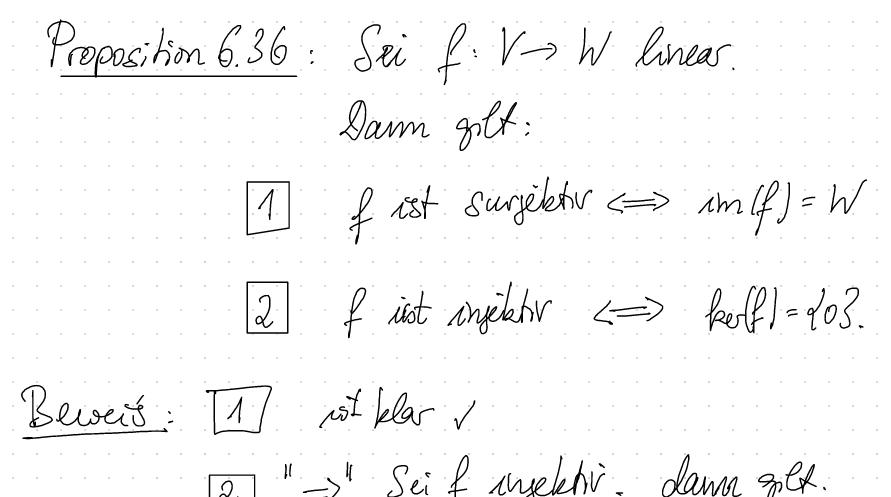
\includegraphics[width=10cm]{./_img/Istklar.jpeg}
        \centering \caption{Beispiel aus der LA1 vom Wintersemester 2020/21 für einen „Beweis“, in dem gar nichts argumentiert wurde. Vgl. die Begründung von \cref{def:surjektiv}.}
    \end{figure}
\end{bem}


\begin{bem}[Subjektivität des Beweisbegriffs]
    Das Wort „überzeugt“ in meiner Beweisdefinition deutet eine subjektive Komponente an. Wenn dich ein Vorlesungs-„Beweis“ nicht überzeugen kann, dann ist er für dich eben auch kein Beweis. Ein Beweistext kann für den Einen eine befriedigende Begründung sein, während er für den Anderen völlig unverständlich und praktisch wertlos ist. Wenn dir unmittelbar klar ist, dass eine Aussage gilt, kann sogar ein „Ist-klar-Beweis“ überzeugend sein.
    
    Nichtsdestotrotz gibt es gewisse Regeln und Techniken, über deren Zulässigkeit ein Konsens besteht. Beweise, die diesen Regeln unterliegen, muss ein Mathematiker anerkennen. Dass Beweise nicht überzeugend sind, kommt so gut wie nie von Verstößen gegen die Logik her; sondern eher von der Verwendung obskurer Begriffe, dem Mangel an Erläuterung komplizierter Beweisschritte, Schreibfehlern, dem Verschleiern von Beweislücken oder oder der unbegründeten Verwendung von Aussagen, die irgendwo fünfzig Seiten vorher einmal in einem unscheinbaren Lemma hergeleitet wurden.
\end{bem}


Bereits in diesem Kapitel werde ich Beweise führen, nämlich um zu demonstrieren, wie sich gewisse logische Schlussregeln und Beweistechniken aus anderen ableiten lassen. Setz dich aber nicht unter Druck, die Herleitungen der Beweistechniken lückenlos nachvollziehen zu müssen, sondern begreife sie als Erklärungen, die plausibel machen sollen, warum die Beweistechniken Sinn ergeben. Letztendlich musst du dich selbst davon überzeugen, wie genau ist gar nicht so wichtig. In den Mathevorlesungen (mal abgesehen von Vorlesungen über Logik, wo es genau darum geht) werden die üblichen Beweistechniken größtenteils ohne weitere Begründung verwendet und ab der zweiten Semesterwoche erwartet auch niemand mehr, dass du die Logik, die deinen Beweisen zugrundeliegt, rechtfertigst (solange sie halt nicht „unlogisch“ ist).





\section{Implikationen}


In diesem Abschnitt seien $A,B$ stets zwei beliebige Aussagen.


\begin{axiom}[Der direkte Beweis] \label{direkterbeweis} \index{Direkter Beweis}
    Um die Aussage „$A\to B$“ zu beweisen, kannst du die Technik des \textbf{direkten Beweises} benutzen:
    
    Nimmt an, dass die Aussage $A$ gilt und zeige nun mithilfe dieser Annahme (und aller weiteren Aussagen, die dir zur Verfügung stehen), dass auch $B$ gilt.
\end{axiom}


\begin{bsp}
    Sofern der FC Bayern München nach dem vorletzten Spieltag bereits vier Punkte vor dem Tabellenzweiten steht, wird er Deutscher Meister.
\end{bsp}


\begin{bew}
    Es sei einmal angenommen, der FC Bayern liege nach dem vorletzten Spieltag vier Punkte vor dem Tabellenzweiten. Weil nur noch ein Spieltag verbleibt, kann der Zweite (und jeder weiter unten stehende Verein) nur noch höchstens drei Punkte im letzten Spieltag gewinnen. Also sind dann die Bayern (schon wieder) uneinholbar und werden Deutscher Meister. \qed
\end{bew}


\begin{bem}[* Zusammenhang zur Interpretation von „$\to$“]
    In \cref{tauto} wurde die folgende Aussage T gezeigt:
    \begin{quote}
        (T): Die Implikation $A\to B$ ist genau dann eine Tautologie, wenn unter jeder (zweiwertigen) Interpretation, unter der $A$ eine wahre Aussage ist, auch $B$ eine wahre Aussage ist.
    \end{quote}
    Dies resultierte aus der Beschaffenheit der Wahrheitstafel für den Implikationspfeil:
    \[\begin{tabular}{cc|c}
        $A$ & $B$ & $A\to B$ \\
        \hline
        w & w & w \\
        w & f & f \\
        f & w & w \\
        f & f & w
    \end{tabular}\]
    Vermittels der Aussage (T) kann diese Wahrheitstafel zur Rechtfertigung der Technik des direkten Beweises verwendet werden. Umgekehrt kannst du aber auch die Technik des direkten Beweises als „natürlicher“ ansehen und die Aussage (T) als Rechtfertigung für die Wahrheitstafel des Implikationspfeils verstehen.
\end{bem}
  
  
\begin{bem}[Signalwörter]
    Wenn du die Implikation $A\to B$ direkt beweist, kannst du dies deutlich machen, indem du den Beweis mit „Es gelte $A$“, „Es sei angenommen, dass $A$ gilt“ oder Ähnlichem beginnst.
\end{bem}

  
\begin{satz}[* Jede Aussage impliziert sich selbst] \label{implikationref}
    Es gilt\footnote{vgl. \cref{teilmengeneig}a)}
    \[ A\to A \]
\end{satz}


\begin{bew}
    Für einen direkten Beweis sei angenommen, dass $A$ gilt. Weil unter dieser Annahme ja $A$ gilt, ist schon alles bewiesen. \qed
\end{bew}

  
\begin{satz}[* Wahres folgt aus Beliebigem]\label{wahresausbeliebigem}
    Es gilt
        \[ A \to (B\to A)   \]
    Mit anderen Worten: Sofern $A$ gilt, wird $A$ auch von $B$ impliziert.
\end{satz}


\begin{bew}
    Für einen direkten Beweis sei angenommen, dass $A$ gilt. Nun ist zu zeigen, dass auch $B\to A$ gilt. Dazu sei zusätzlich angenommen, dass $B$ gilt. Nun gilt auch $A$, weil dies ja schon ganz zu Beginn des Beweises angenommen wurde. \qed
\end{bew}


\begin{bem}[„$\to$“ bedeutet keine Kausalität!]
    Die Aussage, dass Wahres aus Beliebigem folgt, mag seltsam erscheinen (und wird unter die \href{https://de.wikipedia.org/wiki/Paradoxien_der_materialen_Implikation}{Paradoxien der materialen Implikation} gezählt), da dann ja auch Wahres aus solchen Aussagen folgt, die gar nichts damit zu tun haben. Beispielsweise ist „Sofern der Döner in Deutschland erfunden wurde, ist $4$ eine Quadratzahl“ eine wahre Aussage. Dass dies „paradox“ erscheint, kommt von einer inadäquaten Interpretation des Implikationspfeils „$\to$“:
    
    In ihrer üblichsten Interpretation besagt die Aussage $A\to B$ nicht, dass es einen kausalen Zusammenhang zwischen $A$ und $B$ geben muss; sondern nur, dass $B$ unter Annahme von $A$ gilt, egal ob diese Annahme in die Herleitung von $B$ mit einfließt oder nicht. Noch ein Beispiel: Da es, sofern sich das Rad einer Windmühle dreht, windig ist, ist „Wenn sich das Windrad dreht, ist es windig“ eine korrekte Aussage. Aber dies besagt natürlich nicht, dass es windig ist, \emph{weil} sich das Windrad dreht, geschweige denn, dass die Windmühle den Wind erzeugen würde.
\end{bem}


\begin{vorschau}[* Relevanzlogiken]
    Logiken, die sich darum bemühen, dass „$\to$“ wirklich die Bedeutung einer kausalen Implikation trägt, heißen „Relevanzlogiken“, da dort für eine Implikation $A\to B$ gefordert wird, dass $A$ in irgendeiner Hinsicht „relevant“ für $B$ ist. In Relevanzlogiken ist die Technik des direkten Beweises nicht mehr uneingeschränkt zulässig.
\end{vorschau}


\begin{axiom}[Modus ponens] \label{modusponens} \index{Modus Ponens}
    Die logische Schlussregel
    \[\begin{tabular}{r}
        $A\to B$ \\
        $A$ \\
        \hline
        $B$
   \end{tabular}\]
    heißt „Modus ponens“. Sie besagt: Wann immer dir gegeben ist, dass sowohl $A\to B$ als auch $A$ gültig sind, kannst du daraus $B$ schlussfolgern.
\end{axiom}


\begin{bsp}
    Ich habe angekündigt, dass ich, sofern ich zum Bürgermeister gewählt werde, Freibier für alle stiften werde. Sofern ich nun tatsächlich zum Bürgermeister gewählt werde, folgt, dass jedem Freibier ausgeschenkt wird.
\end{bsp}


\begin{bem}[Logik-Latein]
    Du brauchst dir nicht merken, dass diese Schlussregel „Modus ponens“ heißt. Ebensowenig brauchst du dir die anderen lateinischen Bezeichnungen in diesem Vortrag zu merken. Ich gebe die Wörter nur an, um dir das Nachschlagen in Internet und Literatur zu erleichtern.
\end{bem}


\begin{bem}
    \textbf{Vorsicht}: Anfänger machen gelegentlich den Fehler, aus $A\to B$ und $B$ auf die Aussage $A$ zu schließen. Hier ist ein Beispiel für diesen Fehlschluss:
    \begin{quote}
        Sei $x$ eine reelle Zahl. Bekanntlich gilt $(x=3)\to (x^2=9)$. Wenn also tatsächlich $x^2=9$ ist, so muss $x=3$ sein.
    \end{quote}
    Mach dir klar, warum diese Argumentation unzulässig ist.
\end{bem}


\begin{satz}[Direkter Beweis mit Zwischenschritten] \label{implikationtrans}
    Seien $n$ eine natürliche Zahl und $Z_1,\dots , Z_n$ eine Handvoll Aussagen. Um die Implikation $A\to B$ zu beweisen, kannst du die Implikationen
        \[ A\to Z_1,\quad Z_1\to Z_2,\quad \dots ,\quad Z_{n-1}\to Z_n\quad \text{und}\quad Z_n\to B \]
    beweisen.\footnote{vgl. \cref{teilmengeneig}b)} In diesem Fall verwendest du die Aussagen $Z_1,\dots , Z_n$ als \textbf{Zwischenschritte}.
\end{satz}


\begin{bew}
    Es sei angenommen, dass ich alle Implikationen $A\to Z_1$, $Z_1\to Z_2$, \dots , $Z_n\to B$ bewiesen habe. Um zu zeigen, dass dann auch $A\to B$ gilt, sei angenommen, dass $A$ gilt. Wegen $A\to Z_1$ folgt, dass dann auch $Z_1$ gilt. Wegen $Z_1\to Z_2$ folgt, dass auch $Z_2$ gilt. Auf diese Weise können wir schrittweise die $Z$'s durchgehen, sodass am Ende auch $Z_n$ bewiesen ist. Und wegen $Z_n\to B$ gilt dann auch $B$. \qed
\end{bew}


\begin{bsp}
    Falls es nächsten Sommer (schon wieder) zu wenig regnet, wird der Fichtenwald in meiner Heimatstadt gerodet werden.
\end{bsp}


\begin{bew}
    Wenn es nächstes Jahr wieder zu wenig regnet, fehlt es den Fichten an Flüssigkeit, um ausreichend Harz für eine widerstandsfähige Rinde auszubilden. Dies erleichtert es Borkenkäfern, innerhalb der Rinde zu nisten, sodass sich die Borkenkäferpopulation im Wald stark vergrößert und Bäume teilweise absterben werden. Unter diesem Umstand wird die örtliche Forstbehörde beschließen, den Wald zum Schutz vor umstürzenden Bäumen und einer weiteren Ausbreitung der Borkenkäfer zu roden. \qed
\end{bew}

  
\begin{nota}[*]
    Sind $n$ eine natürliche Zahl und $Z_1,\dots , Z_n$ ein paar Aussagen, für die $Z_1\to Z_2, Z_2\to Z_3, \dots, Z_{n-1}\to Z_n$ gilt, so schreibt man auch kurz
        \[ Z_1\to Z_2\to\ \dots\ \to Z_n\]
    Beispielsweise könnte die Argumentation von gerade eben folgendermaßen dargestellt werden:
    \begin{itemize}
        \item[] Nächstes Jahr regnet es zu wenig.
        \item[$\to$] Den Fichten fehlt es an Flüssigkeit, um ausreichend Harz für eine widerstandsfähige Rinde auszubilden.
        \item[$\to$] Borkenkäfern wird es erleichtert, innerhalb der Rinde zu nisten.
        \item[$\to$] Die Borkenkäferpopulation im Wald wird stark vergrößert und Bäume sterben teilweise ab.
        \item[$\to$] Die örtliche Forstbehörde beschließt, den Wald zum Schutz vor umstürzenden Bäumen und einer weiteren Ausbreitung der Borkenkäfer zu roden.   
    \end{itemize}
\end{nota}





\section{Äquivalenzen}


In diesem Abschnitt seien $A,B$ stets zwei beliebige Aussagen.


\begin{axiom}[Hin- und Rückrichtung] \label{hinruck} \index{Hinrichtung} \index{Rückrichtung} \index{Aequivalenzbeweis@Äquivalenzbeweis}
    Aus dem Vorliegen der beiden Implikationen $A\to B$ und $B\to A$ kann auf die Äquivalenz $A\leftrightarrow B$ geschlossen werden.\footnote{vgl. \cref{teilmengeneig}c)}
    \[\begin{tabular}{r}
        $A\to B$ \\
        $B\to A$ \\
        \hline
        $A\leftrightarrow B$
    \end{tabular}\]
    Wenn du die Äquivalenz $A\leftrightarrow B$ beweisen willst, kannst du deinen Beweis also in zwei Teile aufteilen: In der sogenannten \textbf{Hinrichtung} beweist du die Implikation $A\to B$. In der \textbf{Rückrichtung} beweist du die Implikation $B\to A$.
\end{axiom}


\begin{bsp} \label{bsp:hinruck}
    Sei $n$ eine ganze Zahl. Genau dann ist $n$ ein Vielfaches von $6$, wenn es zugleich ein Vielfaches von $2$ und ein Vielfaches von $3$ ist.
\end{bsp}


\begin{bew}
    \begin{enumerate}
        \item[„$\Rightarrow$“:] Sei $n$ ein Vielfaches von $6$. Dies besagt, dass es eine ganze Zahl $k$ mit $n=6\cdot k$ gibt. Es folgt
        \begin{align*}
            n= 2\cdot (3k) \qquad\text{und}\qquad n = 3\cdot (2k)
        \end{align*}
        also ist $n$ sowohl ein Vielfaches von $2$ als auch von $3$.
        \item[„$\Leftarrow$“:] Es sei $n$ sowohl ein Vielfaches von $2$ als auch von $3$. Demzufolge gibt es ganze Zahlen $k,l$ mit
        \begin{align*}
            n = 2k\qquad \text{und}\qquad n  = 3l
        \end{align*}
        Es folgt
        \begin{align*}
            n & = 1\cdot n \\
            & = (3-2)\cdot n \\
            & = 3n - 2n \\
            & = 3\cdot 2k - 2\cdot 3l & (\text{wegen $n=2k$ und $n=3l$})\\
            & = 6k - 6l \\
            & = 6\cdot (k-l)
        \end{align*}
        Also ist $n$ auch ein Vielfaches von $6$. \qed
    \end{enumerate}
\end{bew}


\begin{bem}
    Die Methoden, die in diesen Beweis eingingen, gehören zur „Teilbarkeitstheorie“. Mehr darüber wirst du im zweiten Semester in der Vorlesung „Lineare Algebra 2“ lernen.
\end{bem}


\begin{bem}[Signalwörter]
    Wenn du eine Äquivalenz per Hin- und Rückrichtung beweist, solltest du die jeweiligen Beweisteile mit „$\Rightarrow$“ und „$\Leftarrow$“ beginnen (so wie im Beispiel gerade eben) oder so etwas wie „Ich beweise zuerst die Hinrichtung“ und „Für den Beweis der Rückrichtung sei nun\dots“ schreiben, damit deinem Leser jederzeit klar ist, um welche der beiden Richtungen es gerade geht.
\end{bem}


\begin{axiom}
    Aus der Äquivalenz $A\leftrightarrow B$ kann sowohl auf $A\to B$ als auch auf $B\to A$ geschlossen werden.
    \[\begin{tabular}{r}
        $A\leftrightarrow B$ \\
        \hline 
        $A\to B$ 
    \end{tabular} \qquad\text{und}\qquad \begin{tabular}{r}
        $A\leftrightarrow B$ \\
        \hline 
        $B\to A$ 
    \end{tabular}\]
\end{axiom}


\begin{bsp}
    Es wurde angekündigt, dass man die Prüfung genau dann besteht, wenn man mehr als 50 Punkte erreicht hat. Dann weiß ich einerseits, dass, wenn ich die Prüfung bestanden habe, ich mehr als 50 Punkte erreicht haben muss; andererseits weiß ich, dass ich, sofern ich mindestens 50 Punkte erreicht habe, auf jeden Fall bestanden habe.
\end{bsp}


\begin{satz}[Äquivalenzbeweis mit Zwischenschritten] \label{ifftrans}
    Seien $n$ eine natürliche Zahl und $Z_1,\dots , Z_n$ ein paar Aussagen. Dann kannst du die Äquivalenz $A\leftrightarrow B$ beweisen, indem du die Äquivalenzen
        \[ A\leftrightarrow Z_1,\quad Z_1\leftrightarrow Z_2,\quad \dots,\quad Z_{n-1}\leftrightarrow Z_n \quad\text{und}\quad Z_n\leftrightarrow B \]
    beweist. In diesem Fall agieren die Aussagen $Z_1,\dots , Z_n$ in deinem Beweis als \textbf{Zwischenschritte}.
\end{satz}


\begin{bew}[*]
    \begin{enumerate}
        \item[„$\Rightarrow$“:] Aus den Äquivalenzen $A\leftrightarrow Z_1$, $Z_1\leftrightarrow Z_2$, \dots, $Z_n\leftrightarrow B$ folgen die Implikationen $A\to Z_1$, $Z_1\to Z_2$, \dots, $Z_n\to B$, woraus sich mittels \cref{implikationtrans} ergibt, dass $A\to B$ gilt.
        \item[„$\Leftarrow$“:] Aus den Äquivalenzen $A\leftrightarrow Z_1$, $Z_1\leftrightarrow Z_2$, \dots, $Z_n\leftrightarrow B$ folgen auch die Implikationen $B\to Z_n$, $Z_n\to Z_{n-1}$, \dots, $Z_1\to A$, woraus sich mittels \cref{implikationtrans} auch $B\to A$ ergibt. \qed
    \end{enumerate}
\end{bew}


\begin{nota}
    Sind $n$ eine natürliche Zahl und $Z_1,\dots , Z_n$ ein paar Aussagen, für die $Z_1\leftrightarrow Z_2,\dots, Z_{n-1}\leftrightarrow Z_n$ gilt, so schreibt man auch kurz
    \[ Z_1\leftrightarrow Z_2 \leftrightarrow \ldots \leftrightarrow  Z_n\]
\end{nota}


\begin{bsp}
    Sei $x$ eine positive reelle Zahl. Genau dann ist $x$ eine Lösung der Gleichung $x^2-x=1$, wenn $x= \frac{1+\sqrt{5}}{2}$.\footnote{Die Zahl $\frac{1+\sqrt{5}}{2}$ heißt \href{https://de.wikipedia.org/wiki/Goldener_Schnitt}{Goldener Schnitt}.}
\end{bsp}


\begin{bew}
    Es gilt:
    \begin{alignat*}{3}
        x^2-x& =1 \quad&\leftrightarrow\quad&& \left(x-\frac{1}{2}\right)^2 - \frac{1}{4} &= 1 \\
        && \leftrightarrow\quad&& \left(x-\frac{1}{2}\right)^2&=\frac{5}{4} \\
        && \leftrightarrow\quad&& x-\frac{1}{2} &= \pm \sqrt{\frac{5}{4}} \\
        && \leftrightarrow\quad&& x  &= \frac{1\pm \sqrt{5}}{2} 
    \end{alignat*}
    Weil $x$ positiv ist und $\frac{1-\sqrt{5}}{2}<0$ wäre, ist dies wiederum äquivalent zu $x=\frac{1+\sqrt{5}}{2}$. \qed
\end{bew}


\begin{satz}[* Jede Aussage ist äquivalent zu sich selbst]\label{iffref}
    Es gilt
        \[ A\leftrightarrow A \]
\end{satz}


\begin{bew}
    Mit \cref{implikationref} ist zugleich die Hinrichtung und die Rückrichtung bewiesen. \qed
\end{bew}


\begin{satz}[* Kommutativgesetz für $\leftrightarrow$]\label{iffkomm}
    Es gilt
        \[ (A\leftrightarrow B)\leftrightarrow(B\leftrightarrow A) \]
\end{satz}


\begin{bew}
    \begin{enumerate}
        \item[„$\Rightarrow$“:] Es gelte $A\leftrightarrow B$. Daraus folgt, dass sowohl $A\to B$ als auch $B\to A$ gelten. Das kann natürlich auch andersrum gelesen werden: es gelten sowohl $B\to A$ als auch $A\to B$. Hieraus folgt $B\leftrightarrow A$.
        \item[„$\Leftarrow$“:] Die Rückrichtung beweist man ganz analog zur Hinrichtung, dabei müssen lediglich die Rollen von $A$ und $B$ vertauscht werden. \qed
    \end{enumerate}
\end{bew}


\begin{bem}[Substitutionsprinzip] \index{Substitutionsprinzip}
    Seien $A,B$ zwei äquivalente Aussagen. Dann kannst du in Beweisen die Aussagen $A$ und $B$ beliebig miteinander vertauschen. Möchtest du beispielsweise $A$ beweisen, kannst du genausogut $B$ beweisen. Oder ist dir eine Aussage der Gestalt $(A\land C)\to D$ gegeben, so kannst du genausogut auch mit der Aussage $(B\land C)\to D$ arbeiten.
    
    Aus diesem Grund sind Äquivalenzaussagen wertvoll und nützlich. Sie erlauben es, Aussagen von mehreren Blickwinkeln zu beleuchten und dadurch ein „tieferes“ Verständnis für sie zu gewinnen.
\end{bem}


\begin{satz}[* Curry-Paradoxon\footnote{\href{https://de.wikipedia.org/wiki/Haskell_Brooks_Curry}{Haskell Curry (1900-1982)}}] \label{curryparadox}
    Es gilt
        \[ (A\leftrightarrow (A\to B))\to B \]
    Mit anderen Worten: Ist $A$ bereits äquivalent dazu, dass $B$ von $A$ impliziert wird, so gilt $B$.
\end{satz}


\begin{bew}
    Für einen direkten Beweis sei angenommen, dass $A\leftrightarrow (A\to B)$ gilt. Nun ist zu beweisen, dass $B$ gilt.
    \begin{enumerate}[(1)]
        \item Es gilt $A\to B$, denn: Für einen direkten Beweis sei angenommen, dass $A$ gilt. Wegen $A\leftrightarrow (A\to B)$ gilt dann auch $A\to B$. Und weil $A$ als gültig angenommen wurde, folgt daraus, dass $B$ gilt.
        \item Es gilt $B$, denn: Nach Schritt (1) gilt $A\to B$. Wegen $A\leftrightarrow (A\to B)$ gilt dann auch $A$. Weil nach Schritt (1) auch $A\to B$ gilt, folgt nun, dass auch $B$ gilt. \qed
    \end{enumerate}
\end{bew}


\begin{bem}[* Selbstreferenzielle Aussagen]
    Das Curry-Paradoxon wird deshalb als „Paradoxon“ gehandelt, da es zumindest in der Umgangssprache ziemlich leicht ist, Aussagen $A$ zu konstruieren, für die $A\leftrightarrow (A\to B)$ gilt. Zum Beispiel seien
    \begin{itemize}[labelindent=1.5em, leftmargin=!, labelwidth=\widthof{$B:=$}]
        \item[$A:=$] „Wenn diese Aussage wahr ist, gewinne ich morgen im Lotto.“
        \item[$B:=$] „Morgen gewinne ich im Lotto.“
    \end{itemize}
    Dann gilt tatsächlich $A\leftrightarrow (A\to B)$, sodass aus \cref{curryparadox} folgt, dass ich morgen Millionär bin. Lotterien hassen diesen Trick.
    
    Damit sich mit diesem Trick nicht einfach \emph{jede} mathematische Aussage beweisen lassen kann, muss sichergestellt werden, dass sich die Selbstreferenzialität „Wenn \emph{diese Aussage} wahr ist, dann \dots“, die umgangssprachlich problemlos erzeugbar ist, nicht in formaler mathematischer Sprache nachbilden lässt.
\end{bem}





\subsection*{* Drei häufige Anfängerfehler im Umgang mit Äquivalenzumformungen}


\begin{bem}[„Gleichungs-U's“]
    Aus der Schule sind es manche Studienanfänger gewohnt, Gleichungen dadurch zu beweisen, dass sie sie sovielen Äquivalenzumformungen unterziehen, bis am Ende eine „offensichtliche“ Gleichung rauskommt. Hier ein Beispiel für diese Vorgehensweise:
    \begin{bsp}
    Seien $x,y$ zwei reelle Zahlen. Dann gilt:
        \[ x\cdot (y+1)-x = (x+1)\cdot y-y\]
    \end{bsp}
    \begin{bew}[(Mieser Beweis)]
        Es gilt:
        \begin{alignat*}{3}
            && x\cdot (y+1)-x& \quad=\quad (x+1)\cdot y-y \\
            &\leftrightarrow\qquad& xy + x  -x& \quad=\quad xy + y - y \\
            &\leftrightarrow\qquad& xy & \quad=\quad xy
        \end{alignat*}
    \end{bew}
    Diesen „Beweisstil“ solltest du dir auf keinen Fall aneignen bzw. so bald es geht abgewöhnen! Denn bei so einer Äquivalenzenkette geschieht bei jeder Äquivalenzumformung auf jeder der beiden Seiten eine arithmetische Umformung, die der Leser nachvollziehen muss. Und diese arithmetischen Umformungen bilden den eigentlichen Kern des Beweises, letztendlich hat der Leser die Gleichungskette also in einer „U-Form“, deren beide Stränge erst ganz am Schluss zusammenfinden, zu lesen:
    \[\begin{tikzcd}
        && x\cdot (y+1)-x\ar[red, d, dash] & =& (x+1)\cdot y-y \ar[red, d, dash] \\
        &\leftrightarrow& xy + x-x  \ar[red, d, dash] & =& xy + y - y \ar[red, d, dash] \\
        &\leftrightarrow& xy \ar[red, rr, dash, bend right] & =& xy
    \end{tikzcd}\]
    Schöner ist, es diese Kette arithmetischer Umformungen, gar nicht erst als „U“, sondern als die Kette, als die sie letztendlich auch zu lesen ist, hinzuschreiben:
    \begin{bew}[(Schönerer Beweis)]
        Es gilt:
        \begin{align*}
            x\cdot (y+1) -x& = xy + x -x\\
            & = xy  \\
            & = xy + y - y \\
            & = (x+1)\cdot y -y  &&& \qed
        \end{align*}
    \end{bew}
    Unterscheide dabei sorgfältig von der Art und Weise, wie du den Beweis \emph{findest} und der Art und Weise, wie du ihn am Ende \emph{aufschreibst}\footnote{vgl \cref{rumprobieren} und \cref{beweisaufschreiben}}: Während des Beweisfindungsprozesses ist alles erlaubt und du darfst auf dem Schmierblatt soviele Äquivalenzumformungen aufschreiben, wie du willst. Aber am Ende, wenn es darum geht, den Beweis ansprechend aufzuschreiben, solltest du alle Unsauberkeiten tilgen und den Beweis in eine gut lesbare Form bringen. Ein mathematischer Beweis, wie du ihn in einem Lehrbuch findest oder wie ihn ein Dozent in der Vorlesung vorführt, gibt nur selten den Denkprozess, der seiner Entstehung zugrundelag, wieder. (Was in didaktischer Hinsicht manchmal bedauerlich und einer der Hauptgründe dafür ist, dass sich Erstsemester mit dem Verfassen von Beweisen schwertun.)
\end{bem}


\begin{bem}[Unterschied zwischen $=$ und $\leftrightarrow$]
    Bringe nicht $=$ und $\leftrightarrow$ durcheinander. Die Gleichheit „$=$“ ist eine Beziehung, die zwischen beliebigen Objekten desselben Typs Sinn ergibt. Bspw. ergibt es Sinn zu fragen, ob zwei Zahlen gleich sind, zwei Punkte im Raum gleich sind, zwei Funktionen dieselbe Ableitung haben usw. Dagegen ist „$\leftrightarrow$“ eine Beziehung zwischen \emph{Aussagen}. Manche sind es aus der Schule gewohnt, jegliche Art mathematischen Folgerns durch ein Gleichheitszeichen zu notieren. Die (korrekte) Gleichungsumformung
    \begin{align*}
        x & = y-3 \\
        \leftrightarrow\quad  x+3 & = y
    \end{align*}
    würden sie inkorrekterweise als
    \begin{align*}
        x & = y-3 \\
        = \quad x+3 & = y
    \end{align*}
    notieren, was Leser arg verwirren kann (vor allem, wenn es nicht so schön eingerückt wäre, sondern einfach nur $x=y-3=x+3=y$ dastünde) und auch schlicht mathematisch falsch ist.
    
    Auch hier gilt wieder: In der kreativen Phase, in der du nach einem Beweis suchst und Schmierblatt um Schmierblatt mit Ideen vollschreibst, darfst du Gleichheitszeichen nach Belieben spammen und sogar falsch verwenden. Aber bei der Erstellung des Endprodukts, des Beweises, wie ihn Andere lesen sollen, solltest du penibel auf die korrekte Verwendung von „$=$“'s und „$\leftrightarrow$“'s achten.
\end{bem}


\begin{bem}[Beweise „rückwärts“ führen] \label{hintennachvorne}
    Mal angenommen, ich möchte beweisen, dass die Kubikwurzel von $3$ größer als die Quadratwurzel von $2$ ist. Auf der Suche nach einem Beweis beginne ich einfach mal mit der zu zeigenden Ungleichung $\sqrt[3]{3}>\sqrt{2}$ und forme ein bisschen um:
    \begin{align*}
        && \sqrt[3]{3}& >\sqrt{2} \\
        & \to& \sqrt[3]{3}^{3\cdot 2} & > \sqrt{2}^{2\cdot 3} & (\text{beide Seiten mit $6$ potenzieren}) \\
        & \to & (\sqrt[3]{3}^3)^2 & > (\sqrt{2}^2)^3 & (\text{Potenzgesetz anwenden})\\
        & \to & 3^2 & > 2^3 \\
        & \to & 9 & > 8
    \end{align*}
    Das sieht schonmal gut aus! Durch ein paar Umformungen bin ich auf eine wahre Aussage gelangt. Mancher Anfänger würde nun denken, dass das Problem damit erledigt ist und die obige Ungleichungskette als Beweis taugt.
    
    Das ist aber falsch. Denn die Ungleichungskette beginnt ja mit der zu beweisenden Aussage. Hier wurde also nur die Aussage „Wenn $\sqrt[3]{3} >\sqrt{2}$ gilt, dann ist $9>8$“ bewiesen, die aber leider nichts darüber aussagt, ob nun tatsächlich $\sqrt[3]{3} >\sqrt{2}$ gilt. Glücklicherweise handelt es sich bei allen Umformungen sogar um Äquivalenzumformungen, sodass die Ungleichungskette auch in umgekehrter Richtung gültig ist:
    \begin{align*}
        && 9 & > 8 \\
        & \to & 3^2 & > 2^3 \\
        & \to & (\sqrt[3]{3}^3)^2 & > (\sqrt{2}^2)^3 \\
        & \to& \sqrt[3]{3}^{3\cdot 2} & > \sqrt{2}^{2\cdot 3} & (\text{Potenzgesetz anwenden}) \\
        &\to &  \sqrt[3]{3}& >\sqrt{2}  & (\text{sechste Wurzel ziehen})
    \end{align*}
    Nun ist die Argumentation zumindest mal nicht mehr mathematisch falsch. Wenn ich jetzt noch das „Ungleichungs-U“ loswerde, kann sich der Beweis sehen lassen. Hier ist der finale Beweis:
    \begin{bew}
        Es gilt
        \begingroup
        \allowdisplaybreaks
        \begin{align*}
            \sqrt[3]{3} & = \sqrt[3]{\sqrt{9}} \\
            & = \sqrt[6]{9} \\
            & > \sqrt[6]{8} & (\text{da $\sqrt[6]{-}$ eine ordnungserhaltende Operation und $9>8$ ist}) \\
            & = \sqrt{\sqrt[3]{8}} \\
            & = \sqrt{2} && \qed
        \end{align*}
        \endgroup
    \end{bew}
    Beachte, dass die Struktur dieses Beweises nicht meinen Denkprozess bei der Beweissuche wiederspiegelt. Das ist aber völlig normal und ok. Sollte dein Beweis sehr kompliziert sein, wäre es natürlich trotzdem nett, wenn du, sofern es deinem Leser hilft, ein paar Meta-Bemerkungen darüber, welche Idee hinter dem aktuellen Beweisschritt steckt, einstreust.
    
    Auch Profis stoßen manchmal auf einen Beweis, indem sie die Argumentation „rückwärts“ ausprobieren, also mit der zu beweisenden Aussage starten und schauen, was sich damit anfangen lässt. Während diese Strategie völlig legitim zur Beweis\emph{findung} ist, ist sie es aber nicht zur Beweis\emph{niederschrift}. Dein zum Schluss aufgeschriebener Beweis muss das Problem sauber von den gegebenen Aussagen auf die zu beweisenden Aussagen durchgehen.
    
    Der Versuch, einen Beweis rückwärts zu führen, kann auch Fehler erzeugen, die du, sofern du den Rückwärts-Gedankengang am Ende nicht kritisch reflektierst, übersiehst. Zum Beispiel könnte man meinen, dass für jede reelle Zahl $x$ gilt, dass $\cos(x)=\sqrt{1-\sin^2(x)}$. Denn man kann ja umformen
    \begin{align*}
        &&\cos(x)& =\sqrt{1-\sin^2(x)} \\
        & \to & \cos^2(x)& = 1-\sin^2(x) & (\text{beide Seiten quadrieren}) \\
        & \to & \cos^2(x) + \sin^2(x) &= 1
    \end{align*}
    und letzteres ist eine wohlbekannte wahre Aussage (die manchmal als „Satz des Pythagoras“\footnote{\href{https://de.wikipedia.org/wiki/Pythagoras}{Pythagoras (6. Jhd. v. Chr.)}} bezeichnet wird). Jedoch ist
        \[ \cos(\pi) = -1 \neq 1 = \sqrt{1-0^2} = \sqrt{1-\sin^2(\pi)} \]
    sodass irgendetwas nicht stimmen kann. Kannst du ausmachen, wie und wo genau sich der Fehler eingeschlichen hat?
\end{bem}


\begin{bem}[Weitere Anfängerfehler]
 Eine lange Liste von sowohl studentischen als auch dozentischen Fehlern, die ihm während seiner Lehrtätigkeit aufgefallen sind, hat Eric Schechter auf \href{https://math.vanderbilt.edu/schectex/commerrs/}{seiner Homepage} zusammengetragen.
\end{bem}





\subsection*{* Mehrfach-Äquivalenzen}


\begin{de}[„Die folgenden Aussagen sind äquivalent“] \label{def:tfae}
    Einige mathematische Sätze haben die Gestalt einer größeren Äquivalenzaussage und sehen etwa folgendermaßen aus:
    \begin{quote}
        Es seien \dots und es gelte \dots. Dann sind die folgenden Aussagen äquivalent:
        \begin{itemize}
            \item[(i)] \dots
            \item[(ii)] \dots
            \item[(iii)] \dots
            \item[(iv)] \dots
            \item[\dots]
        \end{itemize}
    \end{quote}
    Diese Satzstruktur kommt so häufig vor, dass sie im Englischen durch ``tfae'' abgekürzt wird (für ``the following are equivalent''). Sie besagt, dass je zwei der Aussagen (i), (ii), (iii), usw. zueinander äquivalent sind, also dass alle Äquivalenzen
        \[ \text{(i)$\leftrightarrow$(ii),\quad (i)$\leftrightarrow$(iii), \quad (ii)$\leftrightarrow$(iii),\quad (i)$\leftrightarrow$(iv),\quad (ii)$\leftrightarrow$(iv), \quad (iii)$\leftrightarrow$(iv),\quad \dots} \]
    gelten. Man sagt auch, die Aussagen seien „paarweise äquivalent“.
 \end{de}
 
 
\begin{bsp}
    Sei $D$ ein Dreieck in der euklidischen Ebene. Dann sind die folgenden Aussagen äquivalent:
    \begin{enumerate}[(i)]
        \item $D$ ist ein gleichseitiges Dreieck, d.h. alle Seiten von $D$ haben dieselbe Länge.
        \item Alle Innenwinkel von $D$ haben dieselbe Größe.
        \item Der Schwerpunkt von $D$ stimmt mit seinem Umkreismittelpunkt überein.
        \item Der Schwerpunkt von $D$ stimmt mit seinem Inkreismittelpunkt überein.
    \end{enumerate}
Würde man hier die Äquivalenz jedes Aussagenpaars per Hin- und Rückrichtung beweisen, müsste man insgesamt zwölf Implikationen beweisen. Mit der folgenden Beweistechnik lässt sich in solchen Fällen erheblich Arbeit einsparen:
\end{bsp}


\begin{satz}[Ringschluss] \label{ringschluss} \index{Ringschluss}
    Seien $n$ eine natürliche Zahl und $A_1,\dots , A_n$ eine Handvoll Aussagen, von denen du beweisen möchtest, dass sie paarweise äquivalent sind. Dann kannst du dies mit der Technik des \textbf{Ringschlusses} erledigen, indem du lediglich die Implikationen
        \[ A_1\to A_2,\quad A_2\to A_3,\quad \dots ,\quad A_{n-1}\to A_n,\quad A_n\to A_1 \]
    beweist. Auf diese Weise „schließt du einen Ring“ zwischen den Aussagen $A_1,\dots , A_n$.
\end{satz}


\begin{bew}
    Durch den Ringschluss wurden alle Implikationen im folgenden Diagramm bewiesen:
    \[\begin{tikzcd}
        &&& A_1 \ar[rrd] &&& \\
        &A_n\ar[rru]&&&& A_2 \ar[ld]& \\
        && \dots \ar[lu] && A_3 \ar[ll]&& 
    \end{tikzcd} \]
    Man sieht, dass sich nun von jeder Aussage mittels Zwischenschritten zu jeder anderen Aussage gelangen lässt, solange man nur lang genug „im Uhrzeigersinn läuft“. Wegen \cref{implikationtrans} gilt daher für je zwei Aussagen $B,C$ aus den $A_1,\dots , A_n$, dass $B\to C$ und $C\to B$, also insgesamt $B\leftrightarrow C$. Demzufolge sind je zwei beliebige Aussagen aus $A_1,\dots , A_n$ zueinander äquivalent. \qed
\end{bew}


\begin{bsp} \label{bsp:ringschluss}
    Sei $n$ eine ganze Zahl. Dann sind die folgenden Aussagen äquivalent:
    \begin{enumerate}[(i)]
        \item Es ist $n\ge 1$.
        \item Für jede ganze Zahl $m$ ist $m+n>m$.
        \item Es gibt mindestens eine ganze Zahl $m$, für die $m+n>m$ gilt.
    \end{enumerate}
\end{bsp}


\begin{bew}
    (i)$\to$(ii): Es gelte (i) und es sei $m$ eine beliebige ganze Zahl. Dann ist
    \begin{align*}
        m+n & \ge m+1 && (\text{wegen (i)}) \\
        & > m
    \end{align*}
    (ii)$\to$(iii) ist trivial, da ganze Zahlen existieren. \\[0.5em]
    (iii)$\to$(i): Es gelte (iii). Dann gibt es eine ganze Zahl $m$ mit $m+n>m$. Subtraktion von $m$ liefert die Ungleichung $n>0$. Und da $n$ eine ganze Zahl ist, muss dann schon $n\ge 1$ gelten. \qed
\end{bew}


\begin{bem}
    \textbf{Achtung}: Ein gelegentlicher Anfängerirrtum besteht darin, zu denken, der Ringschluss müsse \emph{immer} in der Form (i)$\to$(ii), (ii)$\to$(iii), (iii)$\to$(i) durchgeführt werden. Das ist Unsinn und führt dazu, dass sich manche Anfänger einen Haufen unnötige Mehrarbeit aufhalsen.
    
    Genausogut kannst du etwa auch einen Ringschluss über die Implikationen (ii)$\to$(i), (iii)$\to$(ii) und (i)$\to$(iii) durchführen.
    
    Manchmal ist die Ringschluss-Methode auch unangebracht, wenn etwa die beiden Aussagen (ii) und (iii) so widerspenstig gegeneinander sind, dass keine Beweise für (ii)$\to$(iii) und (iii)$\to$(ii) in Sicht sind. In diesem Fall ist es vielleicht einfacher, den scheinbar längeren Weg zu gehen und (i)$\to$(ii), (ii)$\to$(i), (i)$\to$(iii) und (iii)$\to$(i) zu beweisen.
    \[\begin{tikzcd}[column sep=small]
        & (ii) \ar[rd] & \\
        (iii)\ar[ru] && (i)\ar[ll]
    \end{tikzcd}\qquad\text{anstelle von}\qquad\begin{tikzcd}[column sep=small]
        & (i) \ar[rd] & \\
        (iii)\ar[ru] && (ii)\ar[ll]    
    \end{tikzcd}\qquad\text{geht auch.}\]
    \[\text{Manchmal funktioniert aber nur}\qquad \begin{tikzcd}
        & (i) \ar[ld, bend right=20]  \ar[rd, bend right=20] & \\
        (iii)\ar[ru, bend right=20] && (ii) \ar[lu, bend right=20]
    \end{tikzcd}\]
    Entscheidend ist, dass du am Ende so viele Implikationen bewiesen hat, dass man mittels Zwischenschritten von jeder Aussage zu jeder anderen Aussage gelangen kann. \\[0.5em]
    Wenn du eine längere Äquivalenzaussage beweisen möchtest, solltest du immer Ausschau nach Implikationen halten, die „geschenkt“ sind, d.h. deren Beweis besonders naheliegend und einfach ist (in \cref{bsp:ringschluss} war das die Implikation (ii)$\to$(iii)). Daran kannst du dann deine Beweisstrategie orientieren. Ein berüchtigter Äquivalenzbeweis in der LA1-Vorlesung vom Wintersemester 2016/17 verlief so kompliziert, dass der Dozent zu Beginn seines Beweises einen „Plan“ aufgeschrieben hat, um den Studis die Orientierung zu erleichtern.
    \begin{figure}[ht]
        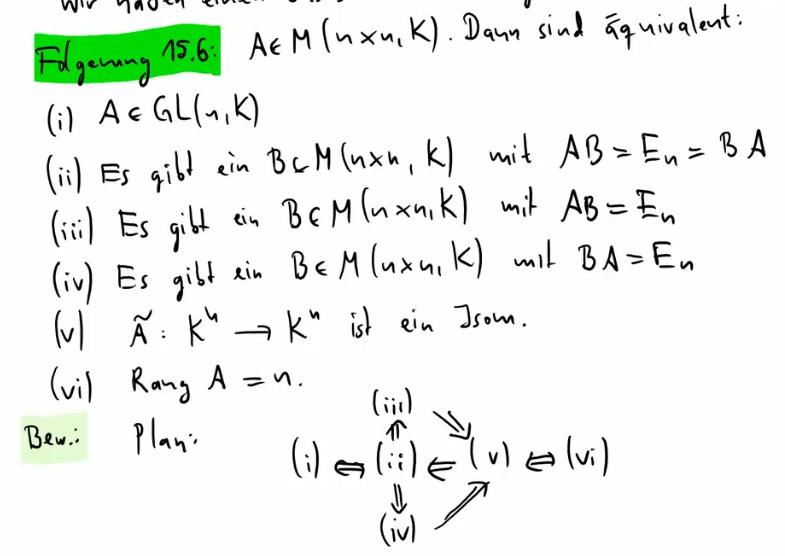
\includegraphics[width=10cm]{./_img/equivbeweis.jpeg}
        \centering \caption{Eine Äquivalenzaussage aus der LA1 vom WS16/17. Hier sind die Implikationen (ii)$\to$(iii) und (ii)$\to$(iv) „geschenkt“.}
    \end{figure}
\end{bem}


\begin{bem}[Signalwörter]
    Wenn du eine Aussage der Gestalt „Folgende Aussagen sind äquivalent\dots“ beweist, solltest du den Beweis jeder einzelnen Implikation mit „(i)$\to$(ii)“, „(iii)$\to$(i)“ oder Ähnlichem betiteln, damit deinem Leser jederzeit klar ist, welche Implikation gerade Thema ist.
\end{bem}





\section{Und und Oder}


In diesem Abschnitt seien $A,B$ stets zwei beliebige Aussagen


\begin{axiom}[*]\label{undoderaxiome}
    Für je zwei Aussagen $A,B$ gelten:
    \begin{align*}
        (A\land B) & \to A & A & \to (A\lor B) \\
        (A\land B) & \to B & B & \to (A\lor B)
    \end{align*}
    Mit anderen Worten: Aus $A\land B$ folgt sowohl $A$ als auch $B$; und $A$ und $B$ sind wiederum hinreichende Bedingungen für $A\lor B$.
\end{axiom}


\begin{bem}
    Wenn dir die Aussage $A\land B$ gegeben ist, kannst du das also so behandeln, als hättest du zwei gegebene Aussagen, nämlich $A$ und $B$.
    
    Und wenn du $A\lor B$ beweisen möchtest, würde es schon reichen, wenn du $A$ beweist oder wenn du $B$ beweist.
\end{bem}


\begin{axiom}[Und-Aussagen beweisen] \label{undbeweise}
    Um die Aussage $A\land B$ zu beweisen, genügt es, sowohl $A$ als auch $B$ zu beweisen:
    \[\begin{tabular}{r}
        $A$ \\
        $B$ \\
        \hline 
        $A\land B$
    \end{tabular} \]
    Mit anderen Worten: Wenn „$A\land B$“ auf deiner „zu zeigen“-Liste steht, kannst du das als zwei separate Ziele behandeln, nämlich musst du einerseits $A$ und andererseits $B$ beweisen.
\end{axiom}


\begin{bsp}[*]
    Die $25$ ist eine Quadratzahl, die sich als Summe zweier echt kleinerer Quadratzahlen schreiben lässt. Außerdem ist sie die kleinste Quadratzahl mit dieser Eigenschaft.
\end{bsp}


\begin{bew}
    (1) Aus
        \[ 25=5^2 \qquad\text{und}\qquad 25 = 9 + 16 = 3^2 + 4^2 \]
    folgt, dass $25$ eine Quadratzahl ist, die sich als Summe zweier echt kleinerer Quadratzahlen schreiben lässt.
    
    (2) Die einzigen Quadratzahlen $\neq 0$, die noch kleiner als $25$ sind, sind
        \[ 1\qquad 4\qquad 9\qquad 16 \]
    Wäre eine dieser vier Zahlen eine Summe zweier echt kleinerer Quadratzahlen, so müssten auch diese beiden Summanden in der Liste dieser vier Zahlen vorkommen. Aber alle möglichen Summationen
    \begin{align*}
        1+1 & = 2 & 1+4 & = 5 \\
        1+ 9 & = 10 & 1+16 & = 17 \\
        4 + 4 & = 8 & 4+9 & = 13 \\
        4+16 & = 20 & 9+9 & = 18
    \end{align*}
    ergeben keine Quadratzahl. \qed
\end{bew}


\begin{bem}[*]
    Drei natürliche Zahlen $a,b,c$, für die $a^2+b^2=c^2$ gilt, heißen ein \textbf{pythagoräisches Tripel}. Also wurde gerade bewiesen, dass $(2,3,5)$ das kleinste pythagoräische Tripel ist. Nach dem berühmten \href{https://de.wikipedia.org/wiki/Gro\%C3\%9Fer_Fermatscher_Satz}{Großen Satz von Fermat}\footnote{\href{https://de.wikipedia.org/wiki/Pierre_de_Fermat}{Pierre de Fermat (1607-1665)}} besitzt die Gleichung $a^n+b^n=c^n$ für eine natürliche Zahl $n\ge 3$ keine positive ganzzahlige Lösung.
\end{bem}


\begin{axiom}[Beweis mit Fallunterscheidung] \label{fallunterscheidung} \index{Fallunterscheidung (in einem Beweis)}
    Sei $X$ eine Aussage, die du beweisen möchtest. Außerdem sei gegeben, dass $A\lor B$ gilt\footnote{Im Englischen sagt man: ``the two cases $A$ and $B$ are \emph{exhausting}''.}. Dann kannst du $X$ mittels einer \textbf{Fallunterscheidung} beweisen, indem du sowohl zeigst, dass $A\to X$ gilt, als auch, dass $B\to X$ gilt.
\end{axiom}


\begin{bsp} \label{bsp:fallunterscheidung}
    Für jede natürliche Zahl $n$ ist $n\cdot (n+1)$ eine gerade Zahl.
\end{bsp}


\begin{bew}
    Da jede natürliche Zahl entweder gerade oder ungerade ist, führe ich eine Fallunterscheidung durch:
    \begin{enumerate}[label={(Fall \arabic*):}, labelindent=1.5em, leftmargin=!, labelwidth=\widthof{(Fall 2):}]
        \item $n$ ist eine gerade Zahl. In diesem Fall ist $n\cdot (n+1)$ als Vielfaches der geraden Zahl $n$ ebenfalls eine gerade Zahl.
        \item $n$ ist eine ungerade Zahl. In diesem Fall ist $n+1$ eine gerade Zahl, sodass $n\cdot (n+1)$ als Vielfaches der Zahl $n+1$ ebenfalls eine gerade Zahl ist.
    \end{enumerate}
    Also ist $n\cdot(n+1)$ in jedem Fall gerade. \qed
\end{bew}





\section{Quantoren}


In diesem Abschnitt sei $E(x)$ stets ein einstelliges Prädikat.


\begin{axiom}[*] \label{quantorenaxiom}
    Sei $a$ irgendein Objekt. Dann gelten die folgenden beiden Implikationen:
    \begin{align*}
         \forall x: E(x) \quad& \to\quad E(a) \\
         E(a) \quad & \to\quad \exists x: E(x)
    \end{align*}
\end{axiom}

 
\begin{bsp}[*] \quad
    \begin{enumerate}
        \item Weil jede positive reelle Zahl eine Qudaratwurzel besitzt, existiert insbesondere auch eine reelle Quadratwurzel der Zwei.
        \item Es existieren $p,q,x,y\in \N_{\ge 1}$ mit $x^p-y^q=1$, denn $3^2-2^3=1$. (Nach dem \href{https://de.wikipedia.org/wiki/Catalansche_Vermutung}{Satz von Catalan-Mihăilescu} gibt es aber keine weiteren Möglichkeiten) 
    \end{enumerate}
\end{bsp}


\begin{satz}[Beweis per Beispiel] \label{beweisperbsp} \index{Beispiel (in einem Beweis)}
    Du kannst die Existenzaussage $\exists x: E(x)$ dadurch beweisen, dass du ein konkretes Objekt $a$ findest, das die Eigenschaft $E$ besitzt. Man nennt dann $a$ ein \textbf{Beispiel} für die Existenzaussage $\exists x: E(x)$.
\end{satz}


\begin{bew}
    Ergibt sich direkt aus der Formel $E(a)\to\exists x:E(x)$. \qed
\end{bew}


\begin{bsp}
    Es gibt eine natürliche Zahl $n\ge 1$, die gleich der Summe ihrer echten Teiler ist.\footnote{Zahlen, die gleich der Summe ihrer echten Teiler sind, heißen auch \href{https://de.wikipedia.org/wiki/Vollkommene_Zahl}{vollkommene Zahlen}.}
\end{bsp}


\begin{bew}
    Ein Beispiel ist die Zahl $28$. Denn die echten Teiler der $28$ sind genau
        \[ 1 \qquad 2 \qquad 4 \qquad 7 \qquad 14 \]
    und es $1+2+4+7+14=28$. \qed
\end{bew}

  
\begin{bem}
    Lässt sich eine Existenzaussage mit einem Beispiel beweisen, so ist es eigentlich schlechter Stil, in einem Buch oder einem Vortrag nur die Existenzaussage anzugeben. Beispielsweise ist ja die Information „Die $24$ ist gleich der Summe ihrer echten Teiler“ umfangreicher als die Information „Es gibt eine natürliche Zahl, die gleich der Summe ihrer echten Teiler ist“. Du solltest dir nicht einfach nur die Existenzaussage merken, sondern, sofern es welche gibt, auch ein paar Beispiele und deren Konstruktion im Hinterkopf behalten. Auch die essenzielle Aussage des Satzes von Euklid \cref{euklid} besteht weniger in der Aussage „Es gibt eine Primzahl, die größer als $n$ ist“ als vielmehr in der trickreichen Art und Weise, wie eine solche Primzahl aufgespürt wird.
    
    Es gibt allerdings auch Situationen, in denen eine Existenzaussage beweisbar ist, obwohl es unmöglich ist, konkrete Beispiele zu geben. Falls in einer Vorlesung keine Beispiele gegeben werden (was bedauerlicherweise recht häufig vorkommt und dem Zeitdruck im Vorlesungsbetrieb zu verdanken ist), solltest du beim Prof. nachhaken, ob er/sie vielleicht deshalb keine Beispiele bringt, weil es gar keine gibt oder die wenigen bekannten Beispiele zu kompliziert und zeitaufwendig sind. Gute Bücher und Vorlesungen erkennt man daran, dass sie, wenn sie keine Beispiele geben, auch erklären, warum.
\end{bem}


\begin{axiom}[Allaussagen an einem „beliebigen“ Objekt nachweisen]\label{allbeweis} \index{beliebig}
    Um die Allaussage $\forall x: E(x)$ zu beweisen, kannst du folgendermaßen vorgehen:
    
    Führe eine Variable $a$, die bislang noch nicht im Beweis verwendet wurde und ein \emph{beliebiges} Objekt bezeichnen soll, ein und beweise nun, dass $a$ die Eigenschaft $E$ besitzt.
\end{axiom}


\begin{bsp} \label{bsp:allbeweis}
    Für jede reelle Zahl $x\neq 1$ existiert eine reelle Zahl $y$ mit $x=\frac{y+1}{y-2}$.
\end{bsp}


\begin{bew}
    Sei $x$ eine beliebige reelle Zahl $\neq 1$. Wegen $x\neq 1$ ist $x-1\neq 0$, sodass durch $y:= \frac{1+2x}{x-1}$ eine wohldefinierte reelle Zahl gegeben ist. Nun rechnet man nach, dass $y\neq 2$ und $\frac{y+1}{y-2}=x$. \qed
\end{bew}

  
\begin{bem}[Signalwörter]
    Ein Beweis einer Allaussage beginnt meist mit Floskeln wie „Sei $x$ ein beliebiges\dots“ oder „Die Zahl $n$ sei beliebig aber fest“. Viele Texte lassen das Signalwort „beliebig“ auch weg und beginnen schlicht mit sowas wie „Sei $x$ eine reelle Zahl. Dann \dots“. Sie setzen vom Leser voraus, dass er erkennt, dass hier gerade der Beweis einer Allaussage beginnt.
\end{bem}
  
 
\begin{bem}[*]
    Achte darauf, dass die von dir eingeführte Variable, die das „beliebige“ Objekt bezeichnen soll, auch wirklich nirgendwo sonst im bisherigen Beweis aufgetaucht ist, also auch wirklich „beliebig“ ist. Ansonsten könnte dir ein Fehler wie der folgende passieren:
    \begin{bsp}[*]
        Es gibt eine natürliche Zahl $n$, die größergleich jede andere natürliche Zahl ist.
    \end{bsp}
    \begin{bew}
        Setze $n=0$. Es bleibt zu zeigen, dass jede natürliche Zahl kleinergleich $n$ ist. Dazu sei $n$ eine beliebige natürliche Zahl. Weil bekanntlich stets $n\le n$ gilt, ist also jede beliebige Zahl kleinergleich $n$.
    \end{bew}
        Ganz so offensichtliche Fehler passieren natürlich eher selten. Subtilere Fehler dieser Art kommen aber durchaus vor.
\end{bem}


\begin{bsp}[* Satz von Euklid\footnote{\href{https://de.wikipedia.org/wiki/Euklid}{Euklid (ca. 3. Jhd. v. Chr.)}}] \label{euklid}
    Für jede natürliche Zahl $n$ gibt es eine Primzahl, die größer als $n$ ist.
\end{bsp}


\begin{bem}
    Die logische Struktur dieses Satzes ist
        \[ \forall\ (\text{natürliche Zahl $n$})\ \exists\ (\text{Primzahl $P$}):\ P>n \]
    Da es sich insgesamt um eine Allaussage handelt, sollte der Beweis mit „Sei $n$ eine beliebige natürliche Zahl“ beginnen. Da daraufhin die Existenzaussage
        \[ \exists P\in \N:\ \text{$P$ ist eine Primzahl und größer als $n$} \]
    übrig bleibt, fährt der Beweis nun mit der geschickten Konstruktion eines Beispiels fort:
\end{bem}


\begin{bew}
    Sei $n$ eine beliebige natürliche Zahl. Da es nur endlich viele natürliche Zahlen gibt, die $\le n$ sind, gibt es auch nur endlich viele Primzahlen, die $\le n$ sind. Seien $k$ deren Anzahl und $p_1,\dots , p_k$ diese Primzahlen. Betrachte die Zahl\footnote{Im Fall $k=0$ ist $N=2$, weil dann ein „leeres Produkt“ involviert ist, siehe \cref{mehrfachprodukt}.}
        \[ N := p_1\cdot\ldots\cdot p_k + 1 \]
    Dann lässt $N$ bei der Division durch $p_1,\dots , p_k$ jedes Mal den Rest Eins übrig, ist also nicht durch $p_1,\dots , p_k$ teilbar. Wegen $N\ge 2$ muss $N$ gemäß dem Fundamentalsatz der Arithmetik aber mindestens einen Primteiler $P$ besitzen. Da $P$ keines der $p_1,\dots ,p_k$ sein kann, aber die $p_1,\dots , p_k$ alle Primzahlen sind, die $\le n$ sind, muss $P$ größer als $n$ sein. \qed
\end{bew}


\begin{axiom}[* Verwenden von Existenzaussagen] \label{exverwendung}
    Sofern dir in einem Beweis eine Aussage der Gestalt $\exists x: E(x)$ gegeben ist, kannst du eine Variable $a$, die bisher noch nirgends im Beweis aufgetaucht ist, einführen, und die Aussage $E(a)$ als gegeben annehmen.
\end{axiom}
  
  
\begin{bsp} \label{bsp:exverwendung}
    Die Gleichung $x^5=x+1$ besitzt eine reelle Lösung.\footnote{vgl. \cref{zeichendefinieren}}
\end{bsp}


\begin{bew}
    Betrachte die reelle Funktion
        \[ f(x) = x^5-x-1 \]
    Dann gilt $f(1)=-1$ und $f(2)=29$. Somit folgt aus dem Zwischenwertsatz der Analysis, dass $f$ eine Nullstelle irgendwo zwischen $1$ und $2$ haben muss. Sei $\xi$ eine solche Nullstelle (hier wird \cref{exverwendung} genutzt). Dann gilt $\xi^5-\xi-1=0$, also $\xi^5=\xi +1$. \qed
\end{bew}


\begin{satz}[* Vertauschbarkeit von Quantoren derselben Sorte] \label{quantorentausch}
    Sei $R$ ein zweistelliges Prädikat. Dann gilt:
    \begin{align*}
        \forall x\ \forall y: R(x,y) \quad &\leftrightarrow\quad \forall y\ \forall x: R(x,y) \\
        \exists x\ \exists y: R(x,y) \quad &\leftrightarrow\quad  \exists y\ \exists x: R(x,y)
    \end{align*}
\end{satz}


\begin{bew}
    Ich beweise jeweils nur die Hinrichtung „$\to$“. Die Rückrichtung wird analog unter Vertauschung der Rollen von $x$ und $y$ bewiesen.
    \begin{itemize}
        \item[„$\forall$“:] Seien $a,b$ zwei beliebige Objekte und es gelte $\forall x\ \forall y: R(x,y)$. Mit \cref{quantorenaxiom} folgt durch Einsetzen von $a$, dass $\forall y: R(a,y)$ und durch Einsetzen von $b$, dass $R(a,b)$. Da $a$ beliebig gewählt war, gilt somit sogar $\forall x: R(x,b)$. Und da auch $b$ beliebig gewählt war, folgt hieraus, dass $\forall y\ \forall x: R(x,y)$.
        \item[„$\exists$“:] Es sei angenommen, dass $\exists x\ \exists y: R(x,y)$ gilt. Dann gibt es ein Objekt $a$, für das $\exists y: R(a,y)$ gilt. Damit gibt es auch ein Objekt $b$, für das $R(a,b)$ gilt. Wegen $R(a,b)$ gilt insbesondere $\exists x: R(x,b)$ und daraus folgt wiederum $\exists y\ \exists x: R(x,y)$. \qed
    \end{itemize}
\end{bew}


\begin{satz}[* Quantoren verschiedener Art sind nicht miteinander vertauschbar!]
    Sei $R$ ein zweistelliges Prädikat. Dann gilt zwar
        \[ \exists x\ \forall y: R(x,y) \quad\to\quad \forall y\ \exists x: R(x,y) \]  
    die umgekehrte Implikation „$\leftarrow$“ ist im Allgemeinen aber falsch, vgl. \cref{quantorreihenfolge}.
\end{satz}


\begin{bew}
    Sei $b$ ein beliebiges Objekt und es gelte $\exists x\ \forall y: R(x,y)$. Dann gibt es ein Objekt $a$, für das $\forall y: R(a,y)$ gilt. Also gilt insbesondere $R(a,b)$. Daraus folgt $\exists x: R(x,b)$ und da das Objekt $b$ beliebig gewählt war, impliziert dies, dass $\forall y\ \exists x: R(x,y)$. \qed
\end{bew}




\subsection*{Eindeutigkeitsbeweise}


Im letzten Vortrag wurde thematisiert, wie sich der Eindeutgikeitsquantor „$\exists !$“ aus dem Allquantor und dem Existenzquantor zusammensetzt:
    \[ \underbrace{\exists x:\ E(x)}_{\text{Es gibt mindestens ein\dots}}\quad \land\quad \underbrace{\forall y,z:\ (E(y)\land E(z)) \to y=z}_{\text{Es gibt höchstens ein\dots}}\]
Diese Und-Aussage kann gemäß \cref{undbeweise} als zwei separate Aussagen behandelt werden:


\begin{satz}[Existenz- und Eindeutigkeitsbeweise] \label{eindbeweis} \index{Eindeutigkeitsbeweis}
    Wenn du eine Aussage der Form $\exists ! x: E(x)$ beweisen möchtest, kannst du deinen Beweis in einen Existenz-Teil und einen Eindeutigkeit-Teil aufteilen:
    \begin{itemize}
        \item Im Existenz-Teil beweist du, dass es mindestens ein Objekt gibt, das die Eigenschaft $E$ besitzt (z.B. durch Angabe eines Beispiels).
        \item Im Eindeutigkeit-Teil beweist du, dass je zwei Objekte, die die Eigenschaft $E$ besitzen, identisch sind.
    \end{itemize}
    Dabei spielt es keine Rolle, ob du erst den Existenz- und dann den Eindeutigkeit-Teil aufschreibst oder umgekehrt.
\end{satz}


\begin{bsp} \label{bsp:eindbeweis}
    Es gibt genau eine reelle Zahl $a$, die für jede reelle Zahl $x$ die Gleichung $a\cdot x=a$ erfüllt.
\end{bsp}


\begin{bew}
    (Eindeutigkeit): Seien $a,b$ zwei reelle Zahlen derart, dass für jede reelle Zahl $x$ gilt, dass $ax=a$ und $bx=b$. Nun ist
    \begin{align*}
        a & = a\cdot b & (\text{wegen der besonderen Eigenschaft von $a$}) \\
        & = b \cdot a  \\
        & = b & (\text{wegen der besonderen Eigenschaft von $b$})
    \end{align*}
    (Existenz): Da für jede reelle Zahl $x$ gilt, dass $0\cdot x=0$, erfüllt die Zahl $0$ die gewünschte Eigenschaft. \qed
\end{bew}


\begin{bem}[Signalwörter]
    Du solltest den Existenz-Teil und den Eindeutigkeit-Teil deines Beweises immer auch als solchen betiteln, so wie es gerade im Beispiel geschah.
\end{bem}


\begin{bem}[Wechselspiel zwischen Formeln und Umgangssprache]
    Anfänger neigen dazu, in ihren Beweisen möglichst alle Sachverhalte in Formelsprache auszudrücken und logische Schritte möglichst rechnerisch, als symbolische Manipulation gewisser Formelterme, durchzuführen. Versuche stattdessen, in deinen Beweisen ein Gleichgewicht aus Formeln und Umgangssprache herzustellen. Wo ein kurzer deutscher Satz dasselbe sagt wie eine Formel, ziehe in Erwägung, den deutschen Satz hinzuschreiben. Gedruckte Beweise (wie etwa in diesem Skript) enthalten oft mehr Fließtext als handschriftliche Beweise (wie sie etwa dein Prof. an die Tafel schreibt).
\end{bem}





\begin{comment}
\section{Induktionsbeweise}


Im Sonderfall, dass sich Allaussagen auf natürliche Zahlen beziehen, stehen Beweistechniken zur Verfügung, die zur Gattung der „Induktionsbeweise“ gehören.


\begin{bem}[Erklärung des Induktionsbeweises]
    Die natürlichen Zahlen lassen sich „abzählen“. Das heißt, wenn ich mit der Null starte und dann anfange zu zählen „Null, Eins, Zwei, Drei,\dots“, so werde ich zwar nie fertig, da es ja unendlich viele Zahlen gibt -- ich werde aber jede beliebige Zahl nach hinreichend langer Zeit abgezählt haben. Mit anderen Worten: Der Zählprozess schöpft die Gesamtheit aller natürlichen Zahlen vollständig aus. Oder: Die Gesamtheit aller natürlichen Zahlen kann durch den Zählprozess „vollständig abgetragen“ werden. \\
    Zählen heißt, mit der Null zu starten und nach jeder genannten Zahl mit der kleinsten noch nicht genannten Zahl fortzufahren. Die natürlichen Zahlen lassen sich also vollständig durch die beiden Operationen
    \begin{itemize}
        \item Mit der Null beginnen.
        \item Sofern man schon ein paar Zahlen abgezählt hat, mit der kleinsten Zahl fortfahren, die noch nicht drankam.
    \end{itemize}
    „abtragen“. Diese Eigenschaft der natürlichen Zahlen liegt dem Prinzip des Induktionsbeweises zugrunde.
\end{bem}


\begin{axiom}[Induktionsbeweis]
    Möchtest du beweisen, dass jede natürliche Zahl die Eigenschaft $E$ besitzt, so kannst du dies folgendermaßen erledigen:
    \begin{itemize}
        \item Im sogenannten \textbf{Induktionsanfang} beweist du, dass $E(0)$ gilt. (Je nach Kontext kann der Induktionsanfang auch bei $n=1$ oder sogar noch höher stattfinden)
        \item Im sogenannten \textbf{Induktionsschritt} fixierst du eine beliebige natürliche Zahl $n\ge 1$ und nimmt an, dass jede Zahl, die kleiner als $n$ ist, die Eigenschaft $E$ besitzt (diese Annehme heißt \textbf{Induktionsannahme} oder auch \textbf{Induktionsvoraussetzung}). Mithilfe dieser Annahme beweist man nun, dass auch $n$ die Eigenschaft $E$ besitzt.
        %\[ \forall n \ge 1:\ (\forall k\le n: E(k)) \to E(n) \]
    \end{itemize}
\end{axiom}


\begin{bsp}[Division mit Rest]
    Seien $a,b$ zwei natürliche Zahlen und $b\neq 0$. Dann gibt es eindeutig bestimmte natürliche Zahlen $q,r$, für die gilt
        \[ a=qb+r \qquad\text{und}\qquad r< b \]
\end{bsp}


\begin{bew}
    (Existenz): Im Fall $a<b$ kann man einfach $q=0$ und $r=a$ setzen. Deshalb sei ab sofort angenommen, dass $a\ge b$ gilt. Der Beweis geschieht nun per Induktion über $a$. \\[0.5em]
    (Induktionsanfang) Im Fall $a=0$ folgt aus $b\neq 0$, dass $a<b$, sodass man einfach $q=0$ und $r=a$ wählen kann. \\
    (Induktionsschritt) Wegen $a\ge b$ ist auch $a-b$ eine natürliche Zahl. Wegen $a-b< a$ gibt es nach Induktionsvoraussetzung eine natürliche Zahl $p$ und eine Zahl $r<b$, für die
        \[ a-b = pb + r \]
    gilt. Setzt man $q:=p+1$, so folgt
        \[ a = (p+1)b + r = qb+r\]
    (Eindeutigkeit): Seien $q,q,r,r'$ natürliche Zahlen mit $r,r'<b$ und $a=qb+r=q'b+r'$. AUSSTEHEND
\end{bew}


\begin{bem}[Signalwörter]
    An diesem Beweis werden eine Reihe wichtiger Punkte deutlich.
    \begin{itemize}
        \item Wenn im Beweis mehrere Variablen vom Typ „natürliche Zahl“ auftreten, musst du deutlich machen, über welche Variable dein Induktionsbeweis verläuft.
        \item Induktionsanfang und Induktionsschritt musst du klar und deutlich kennzeichnen. Deinem Leser muss zu jedem Zeitpunkt klar sein, ob er sich gerade im Induktionsschritt befindet.
        \item Wenn du im Induktionsschritt von der Induktionsannahme Gebrauch musst, musst du das deutlich hervorheben. Diese Stelle ist meist das Herzstück des ganzen Beweises!
    \end{itemize}
\end{bem}


\begin{bem}
    Es gibt einen Haufen Varianten dieser Induktionstechnik. Oftmals wird gar nicht benötigt, dass \emph{alle} kleineren Zahlen als $n$ die Eigenschaft $E$ besitzen und man kann beweisen, dass $E(n)$ allein schon aus $E(n-1)$ folgt. Manchmal führt man den Induktionsanfang auch für $n=1$ oder $n=2$ durch, sofern man etwa sowieso nur beweisen möchte, dass die Eigenschaft für alle Zahlen $\ge 2$ gilt.
    
    Die allgemeine Technik des Induktionsbeweises beschränkt sich nicht nur auf natürliche Zahlen, sondern auf alle möglichen Objekte, die in gewisser Weise „induktiv“ definiert sind. Beispielsweise besagt das \emph{Fundierungsaxiom} der Mengenlehre, dass auch Aussagen über alle Mengen mit einer Induktionstechnik bewiesen werden können. Mehr darüber kannst du in Büchern und Vorlesungen über mathematische Logik und Mengenlehre lernen.
\end{bem}
\end{comment}


\section{Widerlegen}


Alle bisher besprochenen Beweistechniken zielten darauf ab, die „Wahrheit“ von Aussagen zu etablieren. Nun soll es darum gehen, wie man von einer Aussage nachweisen kann, dass sie „falsch“ ist.

In diesem Abschnitt seien $A,B$ stets zwei Aussagen.


\begin{de}[Widerlegung] \index{Widerlegung}
    Eine \textbf{Widerlegung} der Aussage $A$ ist ein Beweis ihrer Negation $\neg A$.
    
    Anstelle von „Es gilt $\neg A$“ schreiben wir auch „$A$ ist falsch“\footnote{Beachte, dass dies erst einmal nichts mit den Wahrheitswerten aus \cref{def:interpretation} zu tun haben muss, vgl. \cref{def:esgilt}}.
\end{de}


\subsection*{Indirekt Argumentieren}


\begin{axiom}[Indirekte Widerlegung] \label{reductio}
    Es gilt:
    \[\begin{tabular}{r}
        $A\to B$ \\
        $\neg B$ \\ \hline
        $\neg A$
    \end{tabular} \]
    Mit anderen Worten: Wenn aus $A$ etwas Falsches folgt, muss $A$ selbst falsch sein.
    
    Du kannst die Aussage $A$ also dadurch widerlegen, dass du eine falsche Aussage $B$ findest, die aus $A$ folgen würde. Man nennt diese Technik eine \textbf{indirekte Widerlegung} oder auch \textbf{Reductio ad absurdum} (latein für „Rückführung auf das Widersinnige“).
\end{axiom}


\begin{bsp} \label{bsp:reductio}
    $198$ ist nicht durch $17$ teilbar.
\end{bsp}


\begin{bew}
    Es ist $187=11\cdot 17$. Wäre $198$ durch $17$ teilbar, so auch die Differenz $198-187 = 11$. Aber $11$ ist kein Vielfaches von $17$. \qed
\end{bew}


\begin{satz}[Widerlegung einer Allaussage per Gegenbeispiel] \label{gegenbeispiel} \index{Gegenbeispiel}
    Wenn du eine Aussage der Gestalt $\forall x: E(x)$ widerlegen möchtest, genügt es, irgendein Objekt $a$ zu finden, für das du $\neg E(a)$ beweisen kannst. Man nennt dann das Objekt $a$ ein \textbf{Gegenbeispiel} zur Allaussage $\forall x: E(x)$.
\end{satz}


\begin{bew}
    Angenommen, du hast $\neg E(a)$ bewiesen. Wegen $(\forall x: E(x)) \to E(a)$ würde dann aus $\forall x:E(x)$ eine falsche Aussage folgen, sodass $\forall x:E(x)$ falsch sein muss. \qed
\end{bew}

 
\begin{bsp}
    Nicht jeder Mensch findet im Leben die große Liebe.
\end{bsp}


\begin{bew}
    Schauen wir uns Franz Schubert an. Mit Mitte Zwanzig an der Syphilis erkrankt, mit 31 Jahren gestorben war es dem Armen nicht leicht gemacht, einen Herzenspartner zu finden. Mehr als kurzzeitige Liebschaften, die er nicht frei ausleben konnte, waren dem Wiener Komponisten zu Lebzeiten nicht vergönnt. Ich meine, hör dir seine \href{https://youtu.be/F6I6Y1LhMKo?t=1665}{Winterreise} nur mal an! -- \qed 
\end{bew}


\begin{satz}[* Implikationen widerlegen]
    Du kannst die Implikation $A\to B$ dadurch widerlegen, dass du beweist, dass $A$ und $\neg B$ gelten.
\end{satz}


\begin{bew}
    Angenommen, es wurden $A$ und $\neg B$ bewiesen. Da $A$ gilt, würde dann aus $A\to B$ die falsche Aussage $B$ folgen. Gemäß \cref{reductio} ist dadurch $A\to B$ widerlegt. \qed
\end{bew}


\begin{bem}[*]
    Die indirekte Widerlegung basiert darauf, dass eine Aussage, aus der etwas Falsches folgt, nicht stimmen kann. Dass aus einer Aussage etwas Wahres folgt, hat dagegen keinerlei Auswirkung, da nach \cref{wahresausbeliebigem} ja Wahres aus Beliebigem folgt.
    
    Betrachte z.B. die (falsche) Aussage $A=$ „Jedes Kind weiß, dass die Summe der Zahlen $1$ bis $100$ gleich $5050$ ist“. Dann folgt aus $A$, dass auch der neunjährige Gauß\footnote{\href{https://de.wikipedia.org/wiki/Carl_Friedrich_Gau\%C3\%9F}{Carl Friedrich Gauß (1777-1855)}} dies wusste, was der \href{https://de.wikipedia.org/wiki/Gau\%C3\%9Fsche_Summenformel#Herkunft_der_Bezeichnung}{Anekdote} zufolge sogar eine wahre Aussage ist. Das ändert allerdings nichts daran, dass $A$ wohl trotzdem falsch ist.
\end{bem}



\begin{de} \index{Kontraposition}
 Die Implikation $\neg B \to \neg A$ heißt die \textbf{Kontraposition} der Implikation $A\to B$. 
\end{de}


\begin{bsp}
    Die Kontraposition der Aussage „Wenn ich krank bin, bleibe ich zuhause“ ist „Wenn ich nicht zuhause bleibe, bin ich nicht krank“.
\end{bsp}


\begin{satz}[Der indirekte Beweis] \label{indirekterbeweis} \index{Indirekter Beweis}
    Die Implikation $\neg A\to \neg B$ kannst du dadurch beweisen, dass du stattdessen die Implikation $B\to A$ beweist. Diese Technik heißt \textbf{indirekter Beweis} oder auch \textbf{Beweis per Kontraposition}.
\end{satz}


\begin{bew}
    Angenommen, es wurde $B\to A$ bewiesen. Dass nun $\neg A\to \neg B$ gilt, zeige ich per direktem Beweis. Dazu sei angenommen, dass $\neg A$ gilt. Wegen $B\to A$ würde dann aus $B$ die falsche Aussage $A$ folgen. Gemäß \cref{reductio} muss also $B$ falsch sein. \qed
\end{bew}


\begin{bsp}
    Sei $n$ eine natürliche Zahl. Sofern $n$ keine Quadratzahl ist, ist auch $n^3$ keine Quadratzahl.
\end{bsp}


\begin{bew}
    Beweis per Kontraposition. Sei $n^3$ eine Quadratzahl, d.h. es gebe eine natürliche Zahl $m$ mit $m^2=n^3$. Es folgt $n=n^3/n^2=m^2/n^2 = (m/n)^2$. Nach dem sogenannten „Satz von der rationalen Nullstelle“ ist jede rationale Zahl, deren Quadrat eine ganze Zahl ist, selbst bereits eine ganze Zahl. Also ist $n=(m/n)^2$ eine Quadratzahl. \qed
\end{bew}
  
  
\begin{bem}[Signalwörter]
    Wenn du einen indirekten Beweis führst, solltest du dies ankündigen, beispielsweise mit „Ich führe einen indirekten Beweis“, „Der Beweis geschieht indirekt“ oder „Beweis per Kontraposition:“.
\end{bem}





\subsection*{Widersprüche}


\begin{de} \index{Widerspruch}
    Ein \textbf{Widerspruch} ist eine Aussage der Gestalt $A\land \neg A$.
\end{de}


\begin{bsp}
    Falls $A$ die Aussage „Schrödingers Katze geht es gut“ ist, so besagt $A\land \neg A$, dass es Schrödingers Katze sowohl gut geht als auch nicht gut geht.
\end{bsp}


\begin{axiom}[Satz vom Widerspruch] \index{Satz vom Widerspruch}
    Für jede Aussage $A$ gilt
        \[ \neg(A\land \neg A) \]
    Mit anderen Worten: Jeder Widerspruch ist eine falsche Aussage.
\end{axiom}


\begin{satz}[Der Widerspruchsbeweis] \label{widerspruchsbeweis} \index{Widerspruchsbeweis}
    Du kannst die Aussage $A$ dadurch wiederlegen, dass du aus ihr einen Widerspruch herleitest. Diese Beweistechnik heißt \textbf{Widerspruchsbeweis}.
\end{satz}


\begin{bew}
    Es sei angenommen, dass aus $A$ ein Widerspruch der Gestalt $B\land \neg B$ folgt. Nach dem Satz vom Widerspruch gilt $\neg (B\land \neg B)$, sodass aus $A$ eine falsche Aussage folgt. Wegen \cref{reductio} ist $A$ somit falsch. \qed
\end{bew}

  
\begin{bsp} \label{bsp:widerspruchsbeweis}
    Unter den positiven reellen Zahlen gibt es keine kleinste.
\end{bsp}


\begin{bew}
    Für einen Widerspruchsbeweis sei angenommen, es gäbe eine kleinste positive reelle Zahl $x$. Da $x$ positiv ist, wäre auch $\frac{x}{2}$ eine positive reelle Zahl. Ferner wäre $\frac{x}{2}<x$. Aber dies widerspräche der Annahme, dass $x$ die kleinste positive reelle Zahl sei. \qed
\end{bew}
  
  
\begin{bem}[* Indirekte Widerlegung vs. Widerspruchsbeweis]
    Meist wird auch die indirekte Widerlegung einer Aussage „Widerspruchsbeweis“ genannt. Aufgrund des Satzes vom Widerspruch ist tatsächlich jeder Widerspruchsbeweis auch eine indirekte Widerlegung (siehe Herleitung von \cref{widerspruchsbeweis}); andererseits kann jede indirekte Widerlegung auch (umständlicherweise) als ein Widerspruchsbeweis formuliert werden, denn mit $A\to B$ und $\neg B$ gilt, da Wahres aus Beliebigem folgt, auch $A\to \neg B$ und somit insgesamt $A\to (B\land \neg B)$.
\end{bem}

  
\begin{bem}[Signalwörter]
    Wenn du dich in einem Widerspruchsbeweis befindest, kannst du, um deinem Leser zu signalisieren, dass du gerade mit \emph{falschen} Aussagen arbeitest, den Konjunktiv II verwenden („dann wäre“, „nun gälte“). Außerdem solltest du die Annahme einer falschen Aussage stets mit „Angenommen, dass\dots“ oder Ähnlichem beginnen. Für den Leser ist es äußerst wichtig zu wissen, zu welchem Zeitpunkt im Beweis es gerade um die Herleitung wahrer Aussagen geht und zu welchem es (um eines Widerspruchsbeweises willen) um die Herleitung falscher Aussagen geht.
    
    Die Stelle im Beweis, an der ein Widerspruch erreicht wird, wird handschriftlich oft mit einem Blitz $\lightning$ markiert. In gedruckten Texten ist der Blitz weniger gängig. Egal wie du es handhabst: du solltest den Moment, an dem du bei einem Widerspruch angelangt bist, stets sprachlich hervorheben.
\end{bem}


\begin{satz}[*] \label{paradox}
    Es gilt
        \[ \neg (A\leftrightarrow \neg A) \]
\end{satz}


\begin{bew}
    Für einen Widerspruchsbeweis sei angenommen, dass $A\leftrightarrow \neg A$ gilt. Daraus folgte $A\to \neg A$ und wegen $A\to A$ gälte dann insgesamt $A\to (A\land \neg A)$. Demnach müsste $A$ falsch sein, d.h. es müsste $\neg A$ gelten. Wegen $A\leftrightarrow \neg A$ folgte aus $\neg A$, dass auch $A$ gälte. Insgesamt läge nun der Widerspruch $A\land \neg A$ vor. \qed
\end{bew}



\begin{bsp}[*] \label{bsp:paradox}
    Aus diesem Grund werden auch Aussagen der Gestalt $A\leftrightarrow \neg A$ gelegentlich als „Widerspruch“ bezeichnet.  Ich persönlich bevorzuge es, Aussagen, die zu ihrer eigenen Negation äquivalent sind, „Paradoxa“ zu nennen.
    \begin{enumerate}
        \item Ein berühmtes Beispiel für eine Aussage, die äquivalent zu ihrer Negation ist, ist das (selbstreferenzielle) \textbf{Lügner-Paradoxon}:
        \begin{quote}
            $A:=$ „Diese Aussage ist falsch.“
        \end{quote}
        Hier gilt tatsächlich $A\leftrightarrow \neg A$.
        \item Eine weitere berühmte Situation, in der eine Aussage äquivalent zu ihrer Negation ist, ist das „Barbier-Paradoxon“, das wiederum ein Spezialfall der sogenannten \emph{Russellschen Antinomie}\footnote{\href{https://de.wikipedia.org/wiki/Bertrand_Russell}{Bertrand Russell 1872-1970}} ist:
        \begin{satz}
            In Sevilla lebt kein Mann, der genau denjenigen Männern Sevillas den Bart rasiert, die sich nicht selbst den Bart rasieren.
        \end{satz}
        \begin{bew}
            Für einen Widerspruchsbeweis sei einmal angenommen, dass es doch einen solchen Mann gäbe. Aus der Beschreibung leitet man ab, dass sich dieser Mann genau dann selbst den Bart rasierte, wenn er ihn sich nicht selbst rasierte. Aber das ist unmöglich. \qed
        \end{bew}
    \end{enumerate}
    
\end{bsp}

  
\begin{satz}[Existenzaussagen widerlegen] \label{existenzwiderleg}
    Sei $E$ eine Eigenschaft. Dann kannst du $\nexists x: E(x)$ dadurch beweisen, dass du $\forall x: \neg E(x)$ beweist.
\end{satz}


\begin{bew}
    Es sei bewiesen, dass $\forall x: \neg E(x)$ gilt. Für einen Widerspruchsbeweis sei nun angenommen, dass dennoch $\exists x: E(x)$ gälte. Dann gäbe es ein Objekt $a$, für das $E(a)$ gälte. Aber wegen $\forall x: \neg E(x)$ gälte auch $\neg E(a)$ und dies ist ein Widerspruch. \qed
\end{bew}


\begin{satz}[* Russellsche Antinomie] \label{russell} \index{Russellsche Antinomie}
    Sei $R$ ein zweistelliges Prädikat, dessen beide Variablen vom selben Typ sind. Dann gilt:
        \[ \nexists x\ \forall y:\ (R(x,y) \leftrightarrow \neg R(y,y))\]
    Mit anderen Worten: Es gibt kein Objekt $x$, sodass jedes Objekt $y$ genau dann in Relation zu $x$ stünde, wenn es nicht in Relation zu sich selbst stünde.
\end{satz}


\begin{bew}
    Für einen Widerspruchsbeweis sei einmal angenommen, es gäbe ein Objekt $a$, für das
        \[ \forall y:\ R(a,y) \leftrightarrow \neg R(y,y) \]
    gälte. Weil es sich hierbei um eine Allaussage handelt, könnten wir für $y$ das Objekt $a$ einsetzen und erhielten die Äquivalenz
        \[ R(a,a) \leftrightarrow \neg R(a,a) \]
    Aber dies ergibt mit \cref{paradox} einen Widerspruch. \qed
\end{bew}
 

\begin{vorschau}[*]
    Definiert man hierbei $R(x,y):\Leftrightarrow$ „$x$ rasiert $y$ den Bart“, so ergibt sich genau das Barbier-Paradoxon aus \cref{bsp:paradox}. Bezeichnen andererseits $x,y$ zwei Mengen und $R(x,y):\Leftrightarrow x\in y$, so erhält man die Aussage, dass es keine Menge gibt, deren Elemente genau diejenigen Mengen sind, die kein Element von sich selbst sind. Diese Aussage war Auslöser der \href{https://de.wikipedia.org/wiki/Grundlagenkrise_der_Mathematik}{Grundlagenkrise} zu Beginn des 20. Jahrhunderts.
\end{vorschau}
  
  

  
    
\section{Aus Falschem folgt Beliebiges}


In diesem Abschnitt seien $A,B$ stets zwei Aussagen.


\begin{axiom}[Modus tollendo ponens] \label{modustp}
    Aus $A\lor B$ und $\neg A$ kannst du schlussfolgern, dass $B$ gilt:
    \[\begin{tabular}{r}
        $A\lor B$ \\
        $\neg A$ \\
        \hline 
        $B$
    \end{tabular} \]
\end{axiom}


\begin{bem}
    Diese Schlussregel kommt bei der Entscheidungsfindung durch Ausschlusskriterien zum Einsatz: Wenn ich weiß, dass von einer Handvoll Aussagen mindestens eine gelten muss, kann ich die wahre Aussage finden, falls ich alle anderen Aussagen ausschließen kann.
\end{bem}


\begin{bsp}
    Ich habe beschlossen, meiner Freundin einen Erdbeerkuchen oder einen Käsekuchen zum Geburtstag zu backen. Falls ich morgen keine Erdbeeren mehr auftreiben kann, werde ich ihr also einen Käsekuchen backen.
\end{bsp}


\begin{satz}[Aus Falschem folgt Beliebiges] \label{exfalso} \index{ex falso quodlibet}
    Es gelten die folgenden beiden Implikationen:
    \begin{align*}
        \neg A & \to (A\to B) \\
        (A\land \neg A) & \to B
    \end{align*}
    Mit anderen Worten: Aus einer falschen Aussage oder einem Widerspruch lässt sich jede beliebige Aussage ableiten. Auf Latein heißt dieses Prinzip \textbf{ex falso quodlibet}.
\end{satz}


\begin{bew}
    Für einen direkten Beweis sei angenommen, dass $\neg A$ und $A$ gelten. Aus $A$ folgt, dass $A\lor B$ gilt, und wegen $\neg A$ muss gemäß \cref{modustp} dann schon $B$ gelten. \qed
\end{bew}


\begin{vorschau}[``principle of explosion''] \label{explosion}
    Da aus Widersprüchen Beliebiges folgt, ist in die Logik eine Art „Bombe“ eingebaut (in der englischen Literatur spricht man sogar vom ``principle of explosion''). Denn wenn es uns gelingen sollte, auch nur eine einzige Aussage sowohl zu beweisen als auch zu widerlegen, folgt aus \cref{exfalso}, dass \emph{jede} beliebige mathematische Aussage beweisbar ist, so unsinnig sie auch sei. Ein solcher Beweis wäre wohl nicht mehr dazu geeignet, die „Wahrheit“ irgendwelcher Aussagen zu etablieren.
    
    Logiken, in denen das ex falso quodlibet nicht gilt, heißen \href{https://ncatlab.org/nlab/show/paraconsistent+logic}{parakonsistente Logiken}. In solchen Logiken hält sich der von Widersprüchen verursachte Schaden in Grenzen und wird teils sogar absichtlich in Kauf genommen; dafür ist dort die Schlussregel aus \cref{modustp} nicht uneingeschränkt anwendbar.
\end{vorschau}





\section{Der Satz vom ausgeschlossenen Dritten}


In diesem Abschnitt seien $A,B$ stets zwei Aussagen.

Die bisherigen Axiome bilden zusammen die sogenannte „intuitionistische“ oder auch „konstruktive“ Logik. Zur sogenannten „klassischen Logik“, die der Mainstream-Mathematik zugrundeliegt, fehlt nur noch das folgende Axiom:


\begin{axiom}[Satz vom ausgeschlossenen Dritten] \label{excludedmiddle} \index{tertium non datur} \index{Satz vom ausgeschlossenen Dritten}
    Es gilt:
        \[ A\lor \neg A \]
    Dieses Prinzip heißt auch \textbf{tertium non datur}, was latein für „ein Drittes kommt nicht vor“ ist. Im Englischen spricht man vom ``principle of excluded middle''.
\end{axiom}


\begin{bsp}
    Sei $A:=$ „Heute ist Mittwoch“. Dann ergibt sich aus dem tertium non datur die Aussage „Heute ist Mittwoch oder heute ist nicht Mittwoch“.
\end{bsp}


\begin{bem}
    Der Satz vom ausgeschlossenen Dritten ist nicht zu verwechseln mit dem Bivalenzprinzip aus \cref{bivalenz}. Das tertium non datur schließt (entgegen seinem Namen -- die Terminologie ist etwas unglücklich) nicht aus, dass es mehr als nur zwei Wahrheitswerte gibt; es besagt lediglich, dass sich die beiden Wahrheitswerte von $A$ und $\neg A$ „in der Summe immer zu `absolut wahr' kombinieren“.
    
    In der philosophischen Logik wird dagegen der Satz vom ausgeschlossenen Dritten mitunter synonym zum Bivalenzprinzip verstanden.
\end{bem}


\begin{bem}[Konsequenz für Fallunterscheidungsbeweise]
    Mit dem tertium non datur stehen uns bedingungslos Oder-Aussagen der Gestalt $A\lor \neg A$ zur Verfügung, die wir für Fallunterscheidungsbeweise einsetzen können. Möchten wir eine Aussage $X$ beweisen und ist $A$ irgendeine beliebige weitere Aussage, so genügt es, $X$ einmal unter der Annahme, dass $A$ gilt, zu beweisen und andererseits unter der Annahme, dass $A$ falsch ist.
    
    Eine der berühmtesten bisher unentschiedenen Aussagen der Mathematik ist die sogenannte \href{https://de.wikipedia.org/wiki/Riemannsche_Vermutung}{Riemannsche Vermutung}\footnote{\href{https://de.wikipedia.org/wiki/Bernhard_Riemann}{Bernhard Riemann (1826 - 1866)}}. Obwohl bislang weder bekannt ist, ob die Vermutung zutrifft oder nicht, konnten \href{https://en.wikipedia.org/wiki/Riemann_hypothesis#Excluded_middle}{diverse Aussagen} dadurch bewiesen werden, dass sie sowohl im Fall, dass die Vermutung zutrifft, gelten, als auch im Fall, dass die Vermutung falsch wäre. Hierbei wird essenziell auf das tertium non datur zurückgegriffen.
\end{bem}


\begin{bsp}
    Es existieren zwei positive irrationale Zahlen $a,b$, für die $a^b$ eine rationale Zahl ist.
\end{bsp}


\begin{bew}
    Ich setze als bekannt voraus, dass $\sqrt{2}$ eine irrationale Zahl ist. Betrachte nun die Aussage
    \begin{quote}
        $A:=$ „$\sqrt{2}^{\sqrt{2}}$ ist eine rationale Zahl.“
    \end{quote}
    Gemäß dem tertium non datur gilt entweder $A$ oder $\neg A$, sodass eine Fallunterscheidung durchgeführt werden kann:
    \begin{itemize}
        \item Falls $A$ gilt, setze einfach $a=b=\sqrt{2}$.
        \item Falls $A$ falsch ist, setze $a=\sqrt{2}^{\sqrt{2}}$ und $b=\sqrt{2}$. Weil $A$ falsch ist, ist $a$ eine irrationale Zahl und es ist
            \[ a^b = (\sqrt{2}^{\sqrt{2}})^{\sqrt{2}} = \sqrt{2}^{\sqrt{2}\cdot\sqrt{2}} = \sqrt{2}^2 = 2 \]
        eine rationale Zahl. \qed
    \end{itemize}
\end{bew}

   
\begin{vorschau}[* Nichtkonstruktivität des tertium non daturs] \label{nichtkonstruktiv} \index{nichtkonstruktiver Beweis}
    Der vorige Beweis ist ein berühmtes Beispiel für einen „nichtkonstruktiven Beweis“. In ihm wird die Existenz zweier Zahlen $a,b$ mit besonderen Eigenschaften bewiesen, ohne dass am Ende des Beweises ein konkretes Beispiel für ein solches Zahlenpaar vorliegt. Zwar wird aus dem Beweis deutlich, dass mindestens eine der beiden Wahlen
    \begin{align*}
        b=\sqrt{2}\ \text{und}\ a=\sqrt{2} \qquad \text{oder}\qquad  b=\sqrt{2}\ \text{und}\ a=\sqrt{2}^{\sqrt{2}}
    \end{align*}
    funktioniert -- welche genau dies ist, bleibt aber im Dunkeln. (Tatsächlich ist $\sqrt{2}^{\sqrt{2}}$ eine irrationale Zahl, sodass $a=\sqrt{2}^{\sqrt{2}}$ gewählt werden muss -- aber dies ist deutlich schwieriger zu beweisen)
    
    Mit dem tertium non datur kommt eine weitere Pathologie auf: In der Mathematik gibt es Aussagen, die, sofern keine Widersprüche herleitbar sind, weder beweisbar noch widerlegbar sind. Die berühmteste dieser „unentscheidbaren“ Aussagen ist vielleicht die \href{https://de.wikipedia.org/wiki/Kontinuumshypothese}{Kontinuumshypothese}. Ist nun $A$ eine unentscheidbare Aussage und ist die Theorie konsistent, so ist weder $A$ noch $\neg A$ beweisbar, obwohl dem tertium non datur gemäß $A\lor \neg A$ gilt. Es liegt also die Situation vor, dass eine Aussage der Gestalt „$X$ oder $Y$“ beweisbar ist, obwohl weder $X$ noch $Y$ beweisbar ist.
    
    In der \emph{intuitionistischen Logik}, die aus allen bisherigen Axiomen mit Ausnahme des tertium non datur besteht, kann dies nicht vorkommen. Mithilfe fortgeschrittener semantischer Methoden lässt sich beweisen, dass sich, sofern sich eine Aussage der Gestalt „$X$ oder $Y$“ ohne Rückgriff aufs tertium non datur beweisen lässt, stets auch schon eine der beiden Aussagen $X$ oder $Y$ beweisen lässt\footnote{Auf Englisch nennt man dies die \href{https://en.wikipedia.org/wiki/Disjunction_and_existence_properties}{``Disjunction property''} der konstruktiven Logik.}. Allerdings lassen sich ohne Rückgriff aufs tertium non datur eben auch weniger Aussagen überhaupt beweisen.
\end{vorschau}

   
\begin{satz}[Regel der doppelten Verneinung] \label{doppelneg}
    Es gilt
    \[ A\leftrightarrow \neg \neg A \]
\end{satz}


\begin{bew}[(*)]
    \begin{itemize}
        \item[„$\Rightarrow$“:] Es gelte $A$. Dann würde aus $\neg A$ sofort der Widerspruch $A\land \neg A$ folgen, sodass $\neg A$ falsch sein muss. Also gilt $\neg\neg A$.
        \item[„$\Leftarrow$“:] Es gelte $\neg \neg A$. Gemäß tertium non datur gilt $A\lor \neg A$. Da $\neg A$ falsch ist, folgt vermöge \cref{modustp}, dass $A$ gelten muss. \qed
    \end{itemize}
\end{bew}


\begin{bem}
    Aufgrund der Regel der doppelten Verneinung kann jede Aussage $A$ mit der verneinenden Aussage $\neg\neg A$ identifiziert werden. Die Aussage $A$ zu beweisen, ist dann gleichwertig dazu, die Aussage $\neg A$ zu widerlegen. Dadurch können alle Widerlegetechniken auch zum Beweis von $A$ eingesetzt werden.
\end{bem}


\begin{satz} \label{implikationchar}
    Es gilt:
        \[ A\to B\quad \leftrightarrow\quad \neg A\lor B \]
\end{satz}


\begin{bew}[(*)]
    \begin{enumerate}
        \item[„$\Rightarrow$“:] Es gelte $A\to B$. Um nun „$\neg A\lor B$“ zu beweisen, mache ich mir das tertium non datur zunutze, demzufolge $A$ oder $\neg A$ gelten muss und führe eine Fallunterscheidung durch:
        \begin{enumerate}[(1)]
            \item Der Fall, dass $A$ wahr ist. In diesem Fall folgt aus der Annahme $A\to B$, dass auch $B$ gilt. Aber dann ist insbesondere auch $\neg A\lor B$ korrekt.
            \item Der Fall, dass $A$ falsch ist. In diesem Fall gilt $\neg A\lor B$ ebenfalls, da ja schon $\neg A$ gilt.
        \end{enumerate}
        Also gilt in jedem Fall $\neg A\lor B$.
        \item[„$\Leftarrow$“:] Es gelte $\neg A\lor B$. Ich werde $A\to B$ direkt beweisen, weshalb einmal angenommen sei, dass $A$ gelte. Aber dann ist $\neg A$ falsch, sodass wegen $\neg A\lor B$ nur noch die Option übrig bleibt, dass $B$ gilt.\footnote{Hier wurde \cref{modustp} benutzt.} \qed
    \end{enumerate}
\end{bew}


\begin{satz}[*] \label{oderperimplikation}
    Möchtest du eine Aussage der Gestalt $A\lor B$ beweisen, so kannst du stattdessen auch $\neg A\to B$ beweisen.
\end{satz}


\begin{bew}
    Es ist
    \begin{align*}
        \neg A\to B \qquad &\leftrightarrow\qquad \neg\neg A\lor B && (\text{wegen \cref{implikationchar}})\\
        & \leftrightarrow\qquad A\lor B && (\text{Regel der doppelten Verneinung}) \qed
    \end{align*}
\end{bew}


\begin{bsp}[*]
    In der Ebene sind zwei Geraden zueinander parallel oder sie schneiden sich in einem Punkt.
\end{bsp}


\begin{bew}
    Wenn zwei Geraden nicht parallel sind, so laufen sie in einer Richtung aufeinander zu. Weil in dieser Richtung der Abstand beider Geraden mit konstanter Rate abnimmt, müssen sich die Geraden in dieser Richtung irgendwann schneiden. \qed
\end{bew}


\begin{satz}[Regeln von De Morgan\footnote{\href{https://de.wikipedia.org/wiki/Augustus_De_Morgan}{Augustus De Morgan (1806 - 1871)}}] \label{demorgan} \index{De Morgansche Regeln}
Es gilt:
    \begin{align*}
        \neg (A\lor B) \quad& \leftrightarrow\quad \neg A\land \neg B \\
        \neg(A\land B) \quad& \leftrightarrow\quad \neg A\lor \neg B
    \end{align*}
\end{satz}


\begin{bew}[(*)]
    Es müssen insgesamt vier Implikationen
    \begin{align}
    \neg (A\lor B) \quad& \to\quad \neg A\land \neg B \tag{1}\\
    \neg A\land \neg B\quad& \to\quad  \neg (A\lor B) \tag{2}\\
    \neg(A\land B) \quad& \to \quad \neg A\lor \neg B \tag{3}\\
    \neg A\lor \neg B \quad& \to \quad \neg(A\land B) \tag{4}
    \end{align}
    bewiesen werden.
    \begin{enumerate}
        \item[(1)] Wegen $A\to (A\lor B)$ und $B\to (A\lor B)$ folgt per Kontraposition, dass $\neg (A\lor B)\to \neg A$ und $\neg(A\lor B) \to \neg B$ gelten muss. Insgesamt folgt nun $\neg(A\lor B)\to( \neg A\land\neg B)$.
        \item[(4)] Wegen $(A\land B)\to A$ und $(A\land B) \to B$ folgt per Kontraposition, dass $\neg A\to \neg(A\land B)$ und $\neg B\to \neg(A\land B)$ gelten muss. Insgesamt folgt nun $(\neg A\lor \neg B)\to \neg(A\land B)$.
        \item[(2)] Sowohl im Fall $A$ als auch im Fall $B$ würde aus $\neg A\land \neg B$ ein Widerspruch folgen. Somit gilt $(A\lor B)\to \neg (\neg A\land \neg B)$. Per Kontraposition folgt daraus $(\neg A\land \neg B) \to \neg(A\lor B)$.
        \item[(3)] Für einen indirekten Beweis sei angenommen, dass $\neg (\neg A\lor\neg B)$ gilt. Mit der (bereits bewiesenen) Implikation (1) folgt daraus, dass $\neg\neg A\land\neg\neg B$ gilt, was mit der Regel der doppelten Verneinung zu $A\land B$ vereinfacht werden kann. \qed
    \end{enumerate}
\end{bew}

 
\begin{satz}[Implikationen per Widerspruch beweisen]
    Um die Implikation $A\to B$ zu beweisen, kannst du folgendermaßen vorgehen: Nimm an, dass sowohl $A$ als auch $\neg B$ gelten und versuche nun, einen Widerspruch herzuleiten.
\end{satz}


\begin{bew}
    Folgt aus der Annahme $A\land \neg B$ ein Widerspruch, so ist damit $\neg(A\land \neg B)$ bewiesen. Wegen
    \begin{align*}
        \neg (A\land \neg B) \quad&\leftrightarrow\quad \neg A\lor \neg\neg B && (\text{Regel von De Morgan}) \\
        &\leftrightarrow\quad \neg A\lor B && (\text{Regel der doppelten Verneinung}) \\
        & \leftrightarrow\quad A\to B && (\text{nach \cref{implikationchar}})
    \end{align*}
    gilt dann auch $A\to B$. \qed
\end{bew}

 
\begin{bem}[Tücken des Widerspruchsbeweises]
    Im Vergleich zum direkten Beweis ist ein Widerspruchsbeweis für $A\to B$ oft leichter zu finden, weil ja eine Annahme mehr als beim direkten Beweis zur Verfügung steht (nämlich $\neg B$). Andererseits sind Widerspruchsbeweise dort, wo auch ein direkter oder indirekter Beweis möglich ist, oft unnötig kompliziert, weshalb du, wenn du einen validen Widerspruchsbeweis gefunden hast, immer noch einmal überprüfen solltest, ob er sich nicht leicht in einen direkten Beweis umformulieren lässt.
    
    Einige Anfänger machen den „Fehler“, ihre Tutoren mit Widerspruchsbeweisen zu überhäufen, wo schon einfachste Modifikationen einen direkten Beweis lieferten (vielleicht weil sie Widerspruchsbeweise mysteriös und cool finden). Allerdings gibt es Situationen, in denen mithilfe metamathematischer Methoden nachgewiesen werden kann, dass ein direkter Beweis unmöglich ist. In solchen Fällen sind Widerspruchsbeweise unvermeidlich.
\end{bem}
  
  
\begin{bsp}[*]
    Ein weiterer Grund dafür, dass du direkte Beweise Widerspruchsbeweisen vorziehen solltest, besteht darin, dass sich Fehler in Widerspruchsbeweisen (wo ja ohnehin mit falschen Aussagen jongliert wird) oft schwieriger ausmachen lassen als in direkten Beweisen. Ein Beispiel:
    \begin{satz}
        Es ist $1=0$.
    \end{satz}
    \begin{bew}[(Unnötig komplizierter Widerspruchs„beweis“)]
        Ich führe einen Widerspruchsbeweis. Dazu nehme ich an, dass $1\neq 0$ und leite daraus einen Widerspruch her.
        
        Wegen $1\neq 0$ ist auch
            \[ 0 = 2\cdot 0 \neq 2\cdot 1 = 2 \]
        und aus $0\neq 2$ folgt $-1\neq 1$. Durch weiteres Umformen kommt man auf
        \begin{align*}
            -1 & \neq 1 \\
            & = \sqrt{1} \\
            & = \sqrt{(-1)\cdot (-1)} \\
            & = \sqrt{-1} \cdot \sqrt{-1} \\
            & = \sqrt{-1}^2 \\
            & = -1
        \end{align*}
        also insgesamt $-1\neq -1$. Aber dies ist eine falsche Aussage. Also muss die Annahme zu Beginn des Beweises, nämlich dass $0\neq 1$ ist, falsch sein. 
    \end{bew}
    Kannst du den Fehler finden? Denk darüber eine Zeitlang nach und versuche daraufhin, den Fehler im folgenden direkten Beweis  zu finden:
    \begin{bew}[(Diesmal als direkter „Beweis“)]
        Es gilt:
        \begin{align*}
            1 & = \sqrt{1} \\
            & = \sqrt{(-1)\cdot (-1)} \\
            & = \sqrt{-1}\cdot \sqrt{-1} \\
            & = \sqrt{-1}^2 \\
            & = -1
        \end{align*}
        also insgesamt $1=-1$. Durch weitere Äquivalenzumformungen folgt:
        \begin{align*}
            1 & = -1 \quad\xrightarrow{+1}\quad 2=0 \quad\xrightarrow{:2}\quad 1=0 
        \end{align*}
    \end{bew}
    Erstsemestern passiert es öfters, dass sie ihre eigenen Denkfehler nur deshalb übersehen, weil ihr Beweis einer unnötig komplizierten Logik unterliegt, mit der sie sich am Ende selbst verwirren. Versuche deshalb, immer den Überblick über deine Beweisstruktur zu behalten und sie so simpel wie möglich zu halten.
\end{bsp}


\begin{satz}[Quantoren negieren] \label{quantorennegieren} \index{Negation von Quantoren}
    Es gilt:
    \begin{align*}
        \nexists x: E(x) \quad& \leftrightarrow\quad \forall x: \neg E(x) \\
        \neg (\forall x: E(x)) \quad& \leftrightarrow\quad \exists x: \neg E(x)
    \end{align*}
\end{satz}


\begin{bew}[(*)]
    Nach Aufteilung in Hin- und Rückrichtungen bleiben insgesamt vier Implikationen übrig, die bewiesen werden müssen:
    \begin{align}
        \neg (\exists x:\ E(x)) \quad& \to\quad (\forall x:\ \neg E(x)) \tag{1} \\
        (\forall x:\ \neg E(x)) \quad& \to\quad \neg (\exists x:\ E(x)) \tag{2} \\
        \neg (\forall x:\ E(x)) \quad& \to\quad (\exists x:\ \neg E(x)) \tag{3} \\
        (\exists x:\ \neg E(x)) \quad& \to\quad \neg (\forall x:\ E(x)) \tag{4}
    \end{align}
    \begin{enumerate}
        \item[(1)] Es gelte $\nexists x : E(x)$. Sei nun $t$ ein beliebiges Objekt. Wegen
            \[ E(t) \quad \to \quad \exists x: E(x) \]
        folgt per Kontraposition, dass $\neg E(t)$ gelten muss. Weil das Objekt $t$ beliebig gewählt wurde, ist damit bewiesen, dass $\forall x: \neg E(x)$ gilt.
        \item[(4)] Ergibt sich aus \cref{gegenbeispiel}.
        \item[(2)] Ergibt sich aus \cref{existenzwiderleg}.
        \item[(3)] Für einen indirekten Beweis sei angenommen, dass $\nexists x: \neg E(x)$ gilt. Mit der (bereits bewiesenen) Implikation (1) folgt daraus, dass $\forall x: \neg\neg E(x)$ gilt, was mit der Regel der doppelten Verneinung zu $\forall x: E(x)$ vereinfacht werden kann. \qed
    \end{enumerate}
\end{bew}


\begin{vorschau}[* Vollständigkeit der erststufigen Prädikatenlogik]
    Jede Formel, die bisher als Axiom gewählt oder hergeleitet wurde, ist eine Tautologie, d.h. wahr unter jeder möglichen (zweiwertigen) Interpretation, siehe \cref{def:interpretation}. Der \emph{Gödelsche Vollständigkeitssatz} besagt auch das Umgekehrte: Jede Tautologie (im Sinne zweiwertiger Interpretationen) lässt sich mithilfe der Axiome und Beweistechniken aus diesem Vortrag herleiten.
    
    Für eine allgemeine Aussage mit Junktoren und Quantoren ist das nicht allzu hilfreich, denn die Beweistechniken dienen uns ja dazu, herauszufinden, welche Aussagen wahr sind -- und nicht etwa dient uns umgekehrt irgendein Wahrheitsorakel dazu, herauszufinden, welche Aussagen beweisbar sind.
    
    Sofern wir es aber mit einer Aussage zu tun haben, die keine Prädikate und Quantoren enthält, sieht die Sache anders aus. Denn für eine solche Aussage, die allein aus den aussagenlogischen Junktoren aufgebaut ist, können wir brute force überprüfen, ob es sich um eine Tautologie handelt, indem wir einen Computer eine Wahrheitstafel ausrechnen lassen und schauen, ob am Ende überall nur w's stehen, siehe \cref{entscheidbar}. Bei komplizierten Aussagen steigt die dafür nötige Rechenkapazität allerdings ins Unermessliche.
\end{vorschau}


\begin{bem}
    Eine Liste mit vielen aussagenlogischen und prädikatenlogischen Tautologien findest du in \cref{formelsammlung}. Wenn du möchtest, kannst du dir einmal zwei oder drei davon raussuchen und versuchen, sie zu beweisen.
\end{bem}





\section{Entstehungsprozess eines Beweises}


Das Schreiben eines mathematischen Beweises gliedert sich grob in drei Phasen, die in diesem Abschnitt einmal durchgegangen werden sollen.  Neben deren abstrakter Beschreibung wird in diesem Abschnitt ein ganz konkretes Beispiel aus der Linearen Algebra entwickelt:


\begin{aufg}
    Gegeben seien die drei Vektoren des $\R^3$:
        \[ v_1:= \begin{pmatrix} 1 \\ 1 \\ 2 \end{pmatrix},\qquad  v_2:= \begin{pmatrix} 2 \\ 1 \\ 0 \end{pmatrix},\qquad v_3:= \begin{pmatrix} 1 \\ 1 \\ 1 \end{pmatrix}\]
    Man beweise, dass $(v_1,v_2,v_3)$ eine Basis des $\R^3$ ist.
\end{aufg}


Möglicherweise wirst du mit diesem Beispiel erst in einigen Wochen etwas anfangen können. Komm dann nochmal hierher zurück.

 
\begin{de}[Phase 1: Recherche]
    In diesem Schritt stellt ihr sicher, euch auf dem Stand der Dinge zu befinden:
    \begin{itemize}
        \item Sofern ihr nicht die Bedeutung aller in der Aufgabenstellung vorkommenden Begriffe kennt, müsst ihr sie im Vorlesungsskript, in eurem Aufschrieb, in einem Lehrbuch oder im Internet nachschlagen. Solange ihr nicht genau wisst, was die Aufgabe besagt, könnt ihr sie nicht lösen.
        \item Mit den Definitionen allein kommt ihr meist aber noch nicht sehr weit. Denn in der Regel wurden in der Vorlesung bereits ein paar praktische Aussagen bewiesen, die ihr euch für eure Lösung zunutze machen könnt. Auf diese Weise bekommt ihr Werkzeuge in die Hand, die ihr in eurem Beweis einsetzen könnt, um euch die Arbeit zu erleichtern. Erstsemestern passiert es nicht selten, dass sie keinen genauen Überblick darüber, was genau in der Vorlesung bewiesen wurde und was nicht, haben, und deshalb unnötige Mehrarbeit verrichten, indem sie unbeabsichtigt versuchen, bereits in der Vorlesung bewiesene Sätze noch einmal selbst zu beweisen.
        \item Ein Problem, das vor allem das erste Studiensemester betrifft, ist, dass gewisse „offensichtliche“ oder bereits aus der Schule bekannte Aussagen für die Lösung der Übungszettel nicht verwendet werden sollen, weil sie noch nicht in der Vorlesung bewiesen wurden. Leider ist im ersten Semester manchmal nicht ganz klar, was man denn nun alles für bekannt voraussetzen darf und wobei es sich um „nichttriviale“ Aussagen, die eines Beweises bedürfen, handelt. Im Zweifelsfall solltet ihr bei eurem Tutor / eurer Tutorin nachfragen. Glücklicherweise hört diese Problematik spätestens im dritten Semester auf.
    \end{itemize}
    Zu dem Beispiel mit den Basisvektoren: Solange ich nicht genau weiß, was eine „Basis des $\R^3$“ ist, kann ich die Aufgabe nicht lösen. Ein Blick in den Vorlesungsaufschrieb verrät mir:
    \begin{quote}
        Das Tripel $(v_1,v_2,v_3)$ ist genau dann eine Basis des $\R^3$, wenn es für jeden Vektor $v\in \R^3$ eindeutig bestimmte reelle Zahlen $a,b,c\in \R$ gibt, für die $v=av_1+bv_2+cv_3$ gilt.
    \end{quote}
    An dieser Definition könnte ich nun meinen Beweisansatz orientieren. Damit würde ich aber unnötige Beweisarbeit verrichten, die bereits in der Vorlesung erledigt wurde. Denn dort wurde die folgende Aussage bewiesen:
    \begin{quote}
        In der Vorlesung wurde bewiesen: Da der $\R^3$ dreidimensional ist, ist $(v_1,v_2,v_3)$ schon dann eine Basis, wenn es linear unabhängig ist.
    \end{quote}
    Dies führt mich auf den Begriff „linear unabhängig“, dessen Bedeutung ich, sofern sie mir nicht absolut klar ist, ebenfalls nachschlagen muss:
    \begin{quote}
        Die Vektoren $(v_1,v_2,v_3)$ heißen \emph{linear unabhängig}, falls für alle $a,b,c\in \R$ mit $av_1+bv_2+cv_3=0$ bereits gelten muss, dass $a=b=c=0$.
    \end{quote}
    Damit habe ich jetzt alle Definitionen beisammen und hoffe, dass ich keinen weiteren Satz aus der Vorlesung, der mir noch mehr Arbeit abnehmen könnte, übersehen habe\footnote{Später in der LA1-Vorlesung wird meist ein „Determinantenkriterium“ bewiesen, mit dessen Hilfe die Aufgabe nochmal erheblich vereinfacht würde.}. Beachte auch, wie mir das Nachschlagen des Vorlesungssatzes Arbeit abgenommen hat. Anfangs hätte ich beweisen müssen, dass es für jeden beliebigen Vektor $v\in \R^3$ eindeutig bestimmte Zahlen $a,b,c\in \R$ mit $v=av_1+bv_2+cv_3$ gibt. Nun muss ich nur noch beweisen, dass diese Zahlen im Fall $v=0$ eindeutig bestimmt sind. Das ist eine erhebliche, unmittelbare Vereinfachung der Aufgabe!
\end{de}


\begin{bem}
    Die Recherchephase ist auch für die Spitzenforschung nicht zu unterschätzen. Probleme im Wissensaustausch sind vielleicht das größte Hindernis mathematischen Fortschritts. So schreibt Peter Johnstone in der Einführung seines Buchs \emph{Stone Spaces} (1982), einem Klassiker der punktfreien Topologie:
    \begin{quote}
        The enormous increase in the number of practising mathematicians since the 1930s has inevitably produced a corresponding decrease in the range of mathematical knowledge that each one possesses on average, and the effect of this is easy to see: theorems and techniques which are commonplace in one field are laboriously and imperfectly rediscovered in adjacent ones.
    \end{quote}
    Gehöre also später nicht zu den Mathematikern, die ihre Zeit damit vergeuden, solche Sätze, die in Fachkreisen längst bewiesen wurden, unter großen Mühen und auch nur halbgar neu zu beweisen, nur weil sie zu schlecht informiert sind; oder den Programmieren, die eine Prozedur furchtbar kompliziert und ineffizient programmieren, nur weil ihnen die frei zugänglichen Bibliotheken unbekannt sind, in denen die Algorithmen bereits hocheffizient implementiert sind. Von diesen Leuten gibt es eine ganze Menge.
\end{bem}


\begin{de}[Phase 2: Rumprobieren] \label{rumprobieren}
    Der zweite Schritt ist die kreativste Phase. Nachdem ihr euch möglichst alle Hilfsmittel, die euch die Vorlesung zum Thema bereitstellt, vergegenwärtigt habt, müsst ihr nun irgendwie einen Beweis aus dem Hut zaubern. Oft werden eure Überlegungen auch dazu führen, dass ihr nochmal zu Phase 1 zurückgeht und weitere Definitionen und Sätze nachschlagt.
    \begin{itemize}
        \item Beleuchtet das Problem von mehreren Seiten. Wenn eine Implikation $A\to B$ zu beweisen ist: seht euch die Kontraposition $\neg B\to \neg A$ an und schaut, ob ihr dadurch eher auf eine Beweisidee kommt. Oder nehmt an, dass sowohl $A$ als auch $\neg B$ gelten und schaut, ob daran irgendetwas faul ist.
        \item In dieser Phase ist wirklich \emph{alles} erlaubt. Ihr könnt völlig ungerechtfertigt irgendwelche Vermutungen aufstellen und mit Hypothesen arbeiten, die euch zwar plausibel erschienen, von denen ihr euch aber gar nicht hundertprozentig sicher seid. Ihr braucht euch hier an keinerlei Logikregeln halten und könnt jeden noch so fernliegenden Bullshit ausprobieren. In dieser Phase betreibt ihr „experimentelle Mathematik“, die nicht logisch fundiert sein muss.
        \item Manchmal kann der Beweis auch „von hinten nach vorne“ durchgeführt werden. D.h. ihr beginnt mit der zu zeigenden Aussage und sucht nach Zwischenschritten, unter deren Annahme ihr die Aussage beweisen könnt\footnote{Für ein Beispiel siehe \cref{hintennachvorne}.}. Dann versucht ihr, diese Zwischenschritte zu beweisen, bis ihr irgendwann bei einer Aussage angekommen seid, die ihr schon an und für sich beweisen könnt. Ich markiere auf meinem Schmierblatt solche Gleichungen, die ich als Hypothesen verwende und die noch „zu zeigen“ sind, mit einem Ausrufezeichen wie etwa
        \begin{align*}
            a,b,c & \stackrel{!}{=} 0 && (\text{lies: „$a,b,c$ sollen gleich $0$ sein“})
        \end{align*}
        Aber ihr dürft in euren Notizen natürlich auch jede andere Art von Kennzeichnung verwenden. Beachtet aber: Während ihr in Phase 2 von hinten nach vorne arbeiten dürft, müsst ihr in Phase 3, wenn es um das Aufschreiben des Beweises geht, so gut es geht „von vorne nach hinten“ arbeiten.
        \item Haltet im Vorlesungsmaterial nach Aussagen ähnlicher Art wie die Aufgabenstellung Ausschau. Möglicherweise könnt ihr Beweistechniken aus der Vorlesung imitieren.
        \item In dieser Phase werdet ihr möglicherweise mehrere Schmierblätter mit für andere Leute völlig unsinnigen, unlesbaren Skizzen vollschreiben. Egal! Es geht hier um \emph{eure} Ideenfindung und erst in der nächsten Phase werdet ihr eure Gedanken für Andere verständlich machen müssen.
        \item Werd im ersten Semester nicht zum Einzelkämpfer! Tausche dich mit deinen Zettelpartnern oder anderen StudentInnen aus! In dieser Phase geht es darum, einen möglichst großen Vorrat an Ideen anzuhäufen, aus dem sich früher oder später die Lösung formen muss. Manchmal hat dein Zettelpartner den entscheidenden Gedanken, der noch fehlt, um deine Strategie aufgehen zu lassen und es wäre dumm und schade, wenn er ihn dir nicht mitteilte. Außerdem kann sich die Gedankenwelt deiner Partner fundamental von deiner eigenen unterscheiden und nur durch Austausch mit Anderen (einschließlich Lehrbücher und Internetseiten) kannst du ein vielseitiges Verständnis für mathematische Objekte gewinnen.
    \end{itemize}
    Diese Phase endet, sobald ihr einen Ansatz gefunden und weiterentwickelt habt, der sich als erfolgreich herausstellt, d.h. von dem ihr euch sicher seid, dass er sich in einen wasserdichten Beweis formulieren lässt. \\[0.5em]
    Zu dem Beispiel mit der Basis im $\R^3$: Die Recherche hat ergeben, dass ich nur noch beweisen muss: Sind $a,b,c\in \R$ drei beliebige reelle Zahlen mit
        \[ a\begin{pmatrix} 1 \\ 1 \\ 2 \end{pmatrix} + b \begin{pmatrix} 2 \\ 1 \\ 0 \end{pmatrix}+c \begin{pmatrix} 1 \\ 1 \\ 1 \end{pmatrix} = 0  \]
    so muss bereits $a=b=c=0$ gelten. Da es sich um eine Gleichung im $\R^3$ handelt, kann ich sie in ein System dreier Gleichungen zerlegen:
    \[\begin{array}{ccccccc}
        a &+& 2b &+& c &=& 0 \\
        a &+& b &+& c & =& 0 \\
        2a && &+ &c & =& 0
    \end{array}\]
    Dieses lineare Gleichungssystem kann ich nun einerseits mit Schulwissen, andererseits mit dem in der LA-Vorlesung präsentierten „Gauß-Algorithmus“ lösen. \\[0.5em]
    Damit ist eine vielversprechende Beweisstrategie gefunden. Auf dem Schmierblatt vergewissere ich mich nun durch ein paar Umformungen, die für nicht-eingeweihte Leser keinen Sinn ergeben müssen, dass das Gleichunssystem tatsächlich auf $a=b=c=0$ führt:
    \begin{align*}
        \leadsto&&   c & = -2a \\
        \leadsto&& -a + b & = 0 \\
        \leadsto&& b& = a \\
        \leadsto&& a +2a-2a & = 0 \\
        \leadsto&& a &= 0 \\
        \leadsto && c & = -2a=0
    \end{align*}
    Damit ist die Aufgabe im Prinzip gelöst. Jetzt muss die Lösung nur noch ordentlich aufgeschrieben werden.
\end{de}
 
 
\begin{de}[Phase 3: Aufschreiben]\label{beweisaufschreiben}
    In dieser Phase geht es darum, einen gut lesbaren Beweistext zu formulieren, der allen Regeln der Kunst genügt. Oftmals werdet ihr in dieser Phase auf Schwächen im Beweis stoßen, die euch dazu zwingen, nochmal in Phase 2 zurückzugehen, um Reparaturen am Beweis durchzuführen.
    \begin{itemize}
        \item Macht euch die logische Struktur eures Beweises deutlich und überlegt euch eine Gliederung der Beweisschritte. Schreibt diese in der Reihenfolge der logischen Argumentationskette auf, nicht in der Reihenfolge der kreativen Ideenkette, die euch auf den Beweis geführt hat, auf. Sollte der Beweis kompliziert sein, solltet ihr aber, sofern es eurem Leser hilft, auch ein paar Meta-Bemerkungen darüber, welche Idee hinter dem aktuellen Beweisschritt steckt, einstreuen.
        \item Sorgt für ein ausgeglichenes Wechselspiel zwischen Formeln und Umgangssprache.
        \item Stellt sicher, dass ihr jede Aussage, die ihr im Beweis verwendet und die nicht völlig naheliegend ist, begründet.
        \item Wenn ihr euch spezielle Aussagen aus der Vorlesung zunutze macht, schreibe so etwas wie „Aus der Vorlesung ist bekannt“ oder „Nach Vorlesung gilt\dots“.
        \item Definitionen aus der Vorlesung braucht ihr nicht noch einmal ausformulieren, sondern ihr könnt voraussetzen, dass euer Tutor / eure Tutorin alle Definitionen, die bislang in der Vorlesung drankamen, kennt. Ebenso könnt ihr alle Variablen, die in der Aufgabenstellung bereits eingeführt wurden, im Beweis verwenden ohne noch einmal neu definieren zu müssen, was sie bedeuten.
        \item Zeige deinen Beweis deinen Zettelpartnern. Wenn sie ihn ohne Zusatzerklärungen nicht verstehen, muss er verbessert werden. Der Beweis muss am Ende selbsterklärend für deinen Tutor / deine Tutorin sein.
        \item Sollte sich herausstellen, dass eure Lösung eine Lücke besitzt, für die euch einfach keine Lösung einfällt -- lasst sie stehen. Ein häufiger Erstsemesterfehler besteht darin, viel zu viel Zeit in die Bearbeitung der Übungszettel zu investieren -- Zeit, die deutlich nützlicher und nachhaltiger darin angelegt wäre, die Vorlesung zu reflektieren, Literatur zu lesen und Freundschaften aufzubauen.
        \item Sollte euer Beweis, wie gerade beschrieben, am Ende noch Lücken enthalten: Seid ehrlich zu euch selbst und eurem Tutor / eurer Tutorin! Ihr werdet mehr Anerkennung und Respekt dafür bekommen, dass ihr in einer kurzen Anmerkung darauf aufmerksam macht, an welcher Stelle noch eine Lücke besteht, und erläutert, woran genau es scheitert, als wenn ihr versucht, eure Lücke mit wirren Formulierungen und komplizierten Formeln zu verschleiern.
    \end{itemize}
    Der letzte Punkt ist vielleicht der allerwichtigste: niemand erwartet, dass ihr von Anfang an perfekte Zettelabgaben produziert! Es ist der Job eures Profs,  eures Tutors und euer selbst, euch mathematisches Arbeiten beizubringen. Falls ihr methodisches oder inhaltliches Unverständnis habt, dürft ihr das nicht verschleiern oder gar euch dafür schämen! Vielmehr solltet ihr versuchen, dieses Unverständnis zu reflektieren und klar auszuformulieren. Das allein ist schon ein schwieriges Vorhaben, für dessen Gelingen ihr Stolz und Anerkennung verdient! \\[0.5em]
    Zu dem Beispiel mit der Basis im $\R^3$: Hier ist ein Beweis, den ich am Ende aufschreiben würde.
    \begin{bew}
        Aus der Vorlesung ist bekannt, dass, da der $\R^3$ ein dreidimensionaler Vektorraum ist, eine Familie dreier Vektoren im $\R^3$ genau dann eine Basis ist, wenn sie linear unabhängig ist. Demnach genügt es zu zeigen, dass $v_1,v_2,v_3$ linear unabhängig sind. \\[0.5em]
        Dazu seien $a,b,c\in \R$ drei beliebige reelle Zahlen mit
            \[ a\begin{pmatrix} 1 \\ 1 \\ 2 \end{pmatrix} + b \begin{pmatrix} 2 \\ 1 \\ 0 \end{pmatrix}+c \begin{pmatrix} 1 \\ 1 \\ 1 \end{pmatrix} = 0  \]
        Man erhält ein lineares Gleichungssystem
        \[\begin{array}{rcccccccc}
            \text{I} &&    a &+& 2b &+& c &=& 0 \\
            \text{II}&& a &+& b &+& c & =& 0 \\
            \text{III} &&  2a && &+ &c & =& 0
        \end{array}\]
        Nun gilt:
        \begin{align*}
            2a+c&=0 \quad \to\quad c = -2a \\
            \xrightarrow[\text{in II einsetzen}]{c=-2a}\quad -a+b &=0 \quad\to\quad b=a \\[0.5em]
            \xrightarrow[\text{in I einsetzen}]{b=a,\ c=-2a} \quad a+2a-2a &= 0 \quad\to\quad a= 0 \\
            \xrightarrow{b=a}\quad b &= 0 \\
            \xrightarrow[c=-2a]{a=0,} \quad c &= 0
        \end{align*}
        Also muss $a=b=c=0$ gelten. Da $a,b,c\in \R$ beliebig gewählt waren, ist damit gezeigt, dass $v_1,v_2,v_3$ linear unabhängig und somit eine Basis sind. \qed
    \end{bew}
\end{de}


Zugegebenermaßen würde ich in einem handschriftlichen Beweisaufschrieb weniger lange Sätze schreiben und mehr mit Einrückungen und Ellipsen arbeiten. Dies lässt sich aber nicht gut in einem gedruckten Text wiedergeben. Beweise in Büchern sehen anders aus als handschriftlich aufgeschriebene Beweise.





\clearpage
\section{Aufgabenvorschläge}


\begin{aufg}[(Un)Logische Schlussfolgerungen]
    Seien $A,B,C$ drei beliebige Aussagen und $E,F,G$ drei Prädikate. Beurteilt die nachfolgenden Schlussfolgerungen danach, ob sie logisch haltbar sind:
    \begin{align*}
        \text{a)}\quad &\begin{tabular}{l}
            Entweder ist der Butler oder der Koch der Mörder. \\
            Entweder ist der Koch oder der Gärtner der Mörder. \\ \hline
            Also gilt: Entweder ist der Butler oder der Gärtner der Mörder.
        \end{tabular} \\[1em]
        \text{b)}\quad &\begin{tabular}{l}
            Im Sterben sagen alle Menschen die Wahrheit. \\
            Im Sterben sagte Siddhartha: „Alles Geschaffene ist vergänglich.“ \\ \hline
            Also gilt: Alles Geschaffene ist vergänglich.
        \end{tabular} \\[1em]
        \text{c)}\quad &\begin{tabular}{l}
            Wenn sich niemand von uns ins Zeug legt, kriegen wir das Projekt nie \\
            \qquad im September fertig. \\
            Wir haben das Projekt im September fertig gekriegt. \\ \hline
            Also gilt: Jeder von uns hat sich ins Zeug gelegt.
        \end{tabular} \\[1em]
        \text{d)}\quad &\begin{tabular}{r}
            $A\to B$ \\
            $C\to \neg B$ \\ \hline
            $A\leftrightarrow \neg C$
        \end{tabular} \\[1em]
        \text{e)}\quad &\begin{tabular}{r}
            $\nexists x:\ F(x)\land G(x)$ \\
            $\forall x:\ E(x)\to F(x)$ \\ \hline 
            $\nexists x:\ E(x)\land G(x)$
        \end{tabular}
    \end{align*}
\end{aufg}



\begin{aufg}[Fehlersuche I]
    Betrachtet den folgenden falschen Satz samt fehlerhaftem Beweis:
    \begin{satz}[Fehlerhafter Satz]
        Seien $x,y$ zwei reelle Zahlen und $x\neq 3$. Gilt dann auch noch $x^2y=9y$, so ist $y=0$
    \end{satz}
    \begin{bew}
        Es gelte $x^2y=9y$. Dann folgt $(x^2-9)y=0$. Wegen $x\neq 3$ ist $x^2\neq 9$, sodass $x^2-9\neq 0$. Daher können wir bei der Gleichung $(x^2-9)y=0$ beide Seiten durch $x^2-9$ teilen und erhalten $y=0$.
    \end{bew}
    \begin{enumerate}
        \item Findet den Fehler im Beweis.
        \item Widerlegt den Satz mit einem Gegenbeispiel.
    \end{enumerate}
\end{aufg}


\begin{aufg}[Fehlersuche II]
    Analysiert den folgenden Satz samt Beweis. Enthält der Beweis Fehler oder Lücken? Stimmt der Satz überhaupt?
    \begin{satz}
        Für jede natürliche Zahl $n$ existiert eine natürliche Zahl $m$, sodass keine der Zahlen $m+1,m+2,\dots , m+n$ eine Primzahl ist. Mit anderen Worten: Es gibt beliebig große Primzahllücken. 
    \end{satz}
    \begin{bew}
        Es sei $n$ eine beliebige natürliche Zahl. Setze 
            \[ m:= (1 \cdot 2 \cdot 3 \cdot \ldots \cdot n \cdot(n+1)) +1 \]
        Dann ist $m+1$ durch $2$ teilbar, $m+2$ durch $3$ teilbar und allgemein $m+k$ durch $k+1$ teilbar für jedes $k\le n$. Also ist keine der Zahlen $m+1,m+2,\dots , m+n$ eine Primzahl. \qed
    \end{bew}
\end{aufg}


\begin{aufg}[Das Dorf der Lügner]
    % --- Der Aufgabentext enthält keine Rechtschreibfehler! ---
    Im beschaulichen Dörfchen Lügenscheid im Sauerland leben genau siebzig Menschen. Jeder dieser Einwohner 
    \begin{itemize}
        \item sagt entweder immer die Wahrheit
        \item oder aber alles was er sagt ist immer gelogen.
    \end{itemize}
    Fasziniert von dieser Begebenheit reist Beate Weiß, eine Mathematik-Doktorandin aus Wahrschau, deren Dissertation im Bereich der angewandten Logik seit Monaten von ihrer Fakultät ausgebremst wird, um sie solange es geht mit prekären befristeten Anstellungen bei der Stange zu halten, in das Dorf, um endlich einen Aufhänger für ihre Arbeit zu finden. Nachdem sie sich im Gasthaus eingerichtet hat, lädt sie alle siebzig Einwohner nacheinander zu einer Befragung ein, bei der sie nur eine einzige Frage stellt: „Wieviele Einwohner dieses Dorfs lügen immer?“
    
    Die erste Person, die zur Befragung erscheint, ein gutmütig aussehender, älterer Herr im Pullunder, sagt ihr, sie müsse sich keine Sorgen machen: im Dorf gebe es nur einen einzigen Lügner -- alle anderen Einwohner sagten dagegen immer die Wahrheit.
    
    Die zweite Person in der Befragung, eine großgewachsene, elegant gekleidete Dame mittleren Alters, sagt ihr, es gebe genau zwei Lügner im Ort.
    
    So geht es immer weiter: Die dritte Person meint, es gebe genau drei Lügner im Dorf, die vierte Person sagt, es gebe genau vier Lügner usw.
    
    Als bereits der Abend angebrochen ist, erscheint endlich auch Einwohner Nummer siebzig, eine greise, etwas orientierungslos wirkende Dame, zur Befragung und krächzt: „Der Teufel soll uns holen. In diesem Dorf gibt es keinen einzigen ehrlichen Menschen. Wir alle sind dazu verflucht, tagein, tagaus zu lügen!“
    
    Frau Weiß ist zufrieden: innerhalb eines Tages ist es ihr gelungen, jeden einzelnen Einwohner des Dorfs zu befragen. Bei einem Bierchen in der Ortskneipe knobelt sie über dem Ergebnis ihrer Studie und versucht herauszufinden, wieviele Lügner es denn nun tatsächlich in Lügenscheid gibt.
    \begin{enumerate}
        \item Findet heraus, wieviele Lügner es in Lügenscheid gibt.
        \item Formuliert einen vollständigen Beweis für eure Behauptung, der keine Bedenken mehr an eurer Antwort übrig lässt.
        \item Analysiert euren Beweis. Welche Techniken (z.B. direkter Beweis, indirekter Beweis, Widerspruchsbeweis, Fallunterscheidung) kommen in eurem Beweis zum Einsatz? Ist der Beweis vielleicht unnötig kompliziert und kann noch vereinfacht werden?
    \end{enumerate}
\end{aufg}

